\part{A Multi-Agent System for Continuous Optimization}\label{MAS4Optim_part}

In the previous part we discussed an inherent limitation of the current continuous optimization approaches. Not only are the current methods highly specialized, but they are also limited by the size, and ultimately by the complexity of the problem. The most complex problems require specific approaches (MDO methods) in order to distribute this complexity while keeping a coherent view. However, these approaches are often complicated to put in practice and tend themselves to be specialized to certain problem types.

In this part we present the main contribution of this thesis: a novel approach to solve complex continuous optimization problems using a MAS. We start by creating a new modeling of continuous optimization problems as entities graphs, and agentify these entities to produce a MAS. We then design agent behaviors and specific mechanisms for the MAS to be able to solve the optimization problem in a distributed way, while maintaining a coherent view of the problem by propagating messages from neighbors to neighbors. 

First we propose a new way to model a continuous optimization as a MAS. We want our modeling must be general enough to allow any continuous optimization problem to be transformed in such a way. We also want it simple enough to be automated, which is not only a requirement in the case of big problems, but also a way for the MAS to work \enquote{behind the scenes}, without requiring the user of the system to have a specific knowledge of multi-agent related concepts. Since optimization specialists often possess expert knowledge and techniques associated to the problems they want to solve, we would like our modeling to be able to integrate with external optimization tools. Our last requirement is to allow the persons in charge of the optimization process to be able to express the problem in the formulation which is the most natural for them, without requiring the problem to be reformulated in any way.

After presenting our modeling, we design an agent-based algorithm for the solving of complex continuous optimization problems. We expose the basic, nominal workflow of the system, how the agents try to optimize the different parts of the system and exchange inform and request messages in order to propagate changes and coordinate the optimization process. We then see how specific configurations related to complex continuous optimization problems can cause this nominal optimization workflow to fail. Using the AMAS theory, we categorize these configurations into different non cooperative situations. For each of these NCSs we propose additional cooperative mechanisms in order to detect, solve the NCS and re-establish the correct optimization process.

At last, we see how our agent modeling can be extended, by proposing some modifications in our system to take in account the handling of uncertainties during the optimization process. We first see how the expression of the problem is changed by the integration of uncertainties. We modify the structure of the information exchanged by the agents and identify some key operations they require in order to be able to manipulate exchanged data. Finally we propose a generic mechanism for experts to be able to express how different representations of uncertainties can be propagated in the context of the problem to solve.

\chapter{Agent-Based Modeling and Simulation of a Continuous Optimization Problem}

\section{NDMO: A Natural Domain Modeling for Optimization}\label{modeling}

As we previously stated, when solving complex continuous problems existing techniques (\emph{i.e.} MDO methods) usually require a transformation of the initial formulation, in order to satisfy some requirements for the technique to be applied. Beside the fact that correctly applying these changes can be a demanding task for the designers, imposing such modifications changes the problem beyond its original, natural meaning. What we propose here is an agent-based modeling where the original structure, the original meaning of the problem is preserved, because it represents the formulation which is the most natural and easiest for the expert to manipulate. This modeling decomposes the elements of the problem into a graph of entities, which can then be instantiated as agents. We call this modeling \emph{Natural Domain Modeling for Optimization} (NDMO).

\begin{figure}[]
	\centering
	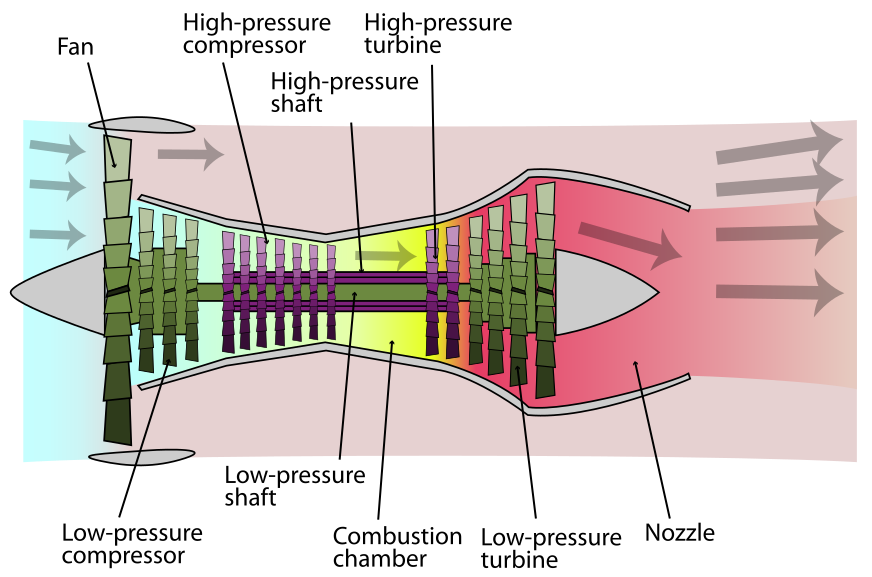
\includegraphics[width=0.75\textwidth]{Turbofan_operation}
	\caption{Illustration of a Turbofan engine (CC SA-BY \href{http://en.wikipedia.org/wiki/File:Turbofan_operation.svg}{K. Aainsqatsi}).}
	\label{turbofan_illu}
\end{figure}

To illustrate how an optimization problem is modeled with NDMO, we use the example of a simplified turbofan optimization problem. On \figurename{} \ref{turbofan_illu}, an illustration of the principle of the turbofan can be seen. On such engine, we call bypass ratio the ratio between the air drawn in by the fan not entering engine core (which is \emph{bypassed}) and the air effectively used for the combustion process. We also call pressure ratio the ratio between pressure produced by the compressors and the pressure it receives from the environment.

In order to identify the elements of a generic continuous optimization model, we worked with experts from several related fields: numerical optimization, mechanics as well as aeronautics and engine engineers. As a result, we identified five classes of interacting entities: \emph{models}, \emph{design variables}, \emph{outputs}, \emph{constraints} and \emph{objectives}. These entities and their relations are represented by the diagram in \figurename{} \ref{class_diag}, that we detail next.

\begin{figure}[t]
	\centering
	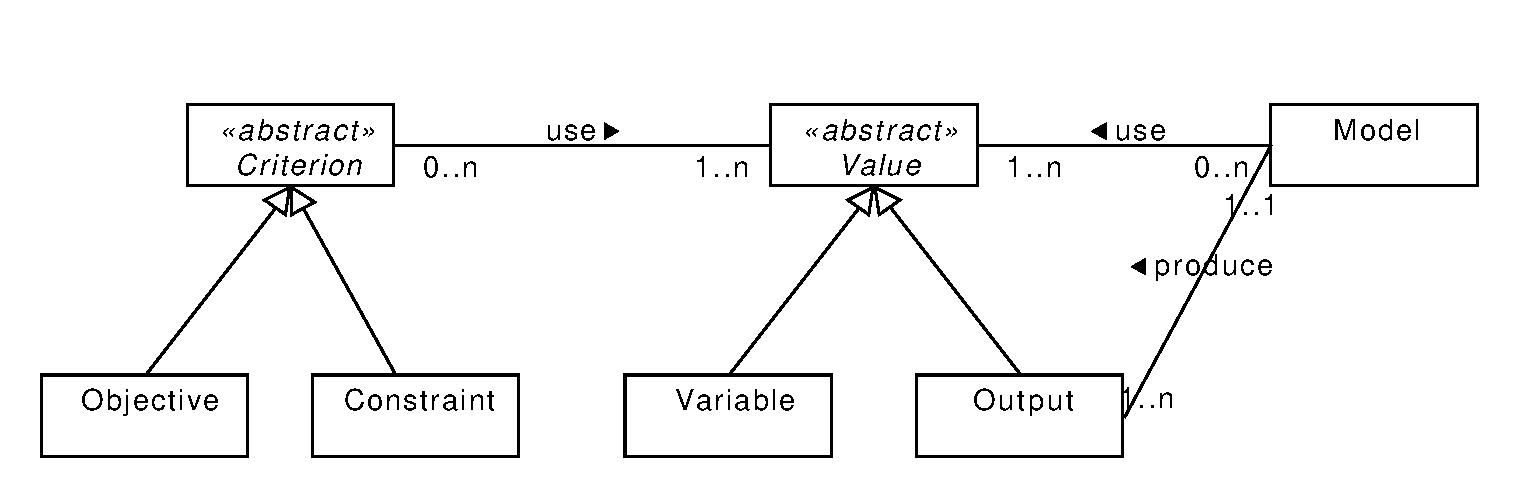
\includegraphics[width=0.9\textwidth]{class_diag}
	\caption{Class diagram of MDO problems.}
	\label{class_diag}
\end{figure}

On \figurename{} \ref{turbofan:math}, the analytic expression of this optimization problem is given, while on \figurename{} \ref{turbofan:graph}, the problem is presented as a graph of the different entities. The design variables of this problem are $pi\_c$ and $bpr$, which indicate respectively the compressor pressure ratio and the bypass ratio of the engine. The turbofan model produces three outputs: $Tdm0$, $s$ and $fr$, representing respectively the thrust, fuel consumption and thrust ratio of the engine. In this problem we try to maximize the thrust and minimize the fuel consumption while satisfying some feasibility constraints. 

\begin{figure}
\centering
	\begin{subfigure}[b]{0.4\textwidth}
		$\begin{array}{c}
			(Tdm0, s, fr) = Turbofan(pi\_c, bpr) \\
			max \; Tdm0 \\
			min \; s \\
			subject \; to \\
			s \leq 155 \\
			fr \geq 4
		\end{array}$
		\caption{mathematical formulation.}\label{turbofan:math}
	\end{subfigure}
	\hfill%
	\begin{subfigure}[b]{0.55\textwidth}
			\centering
			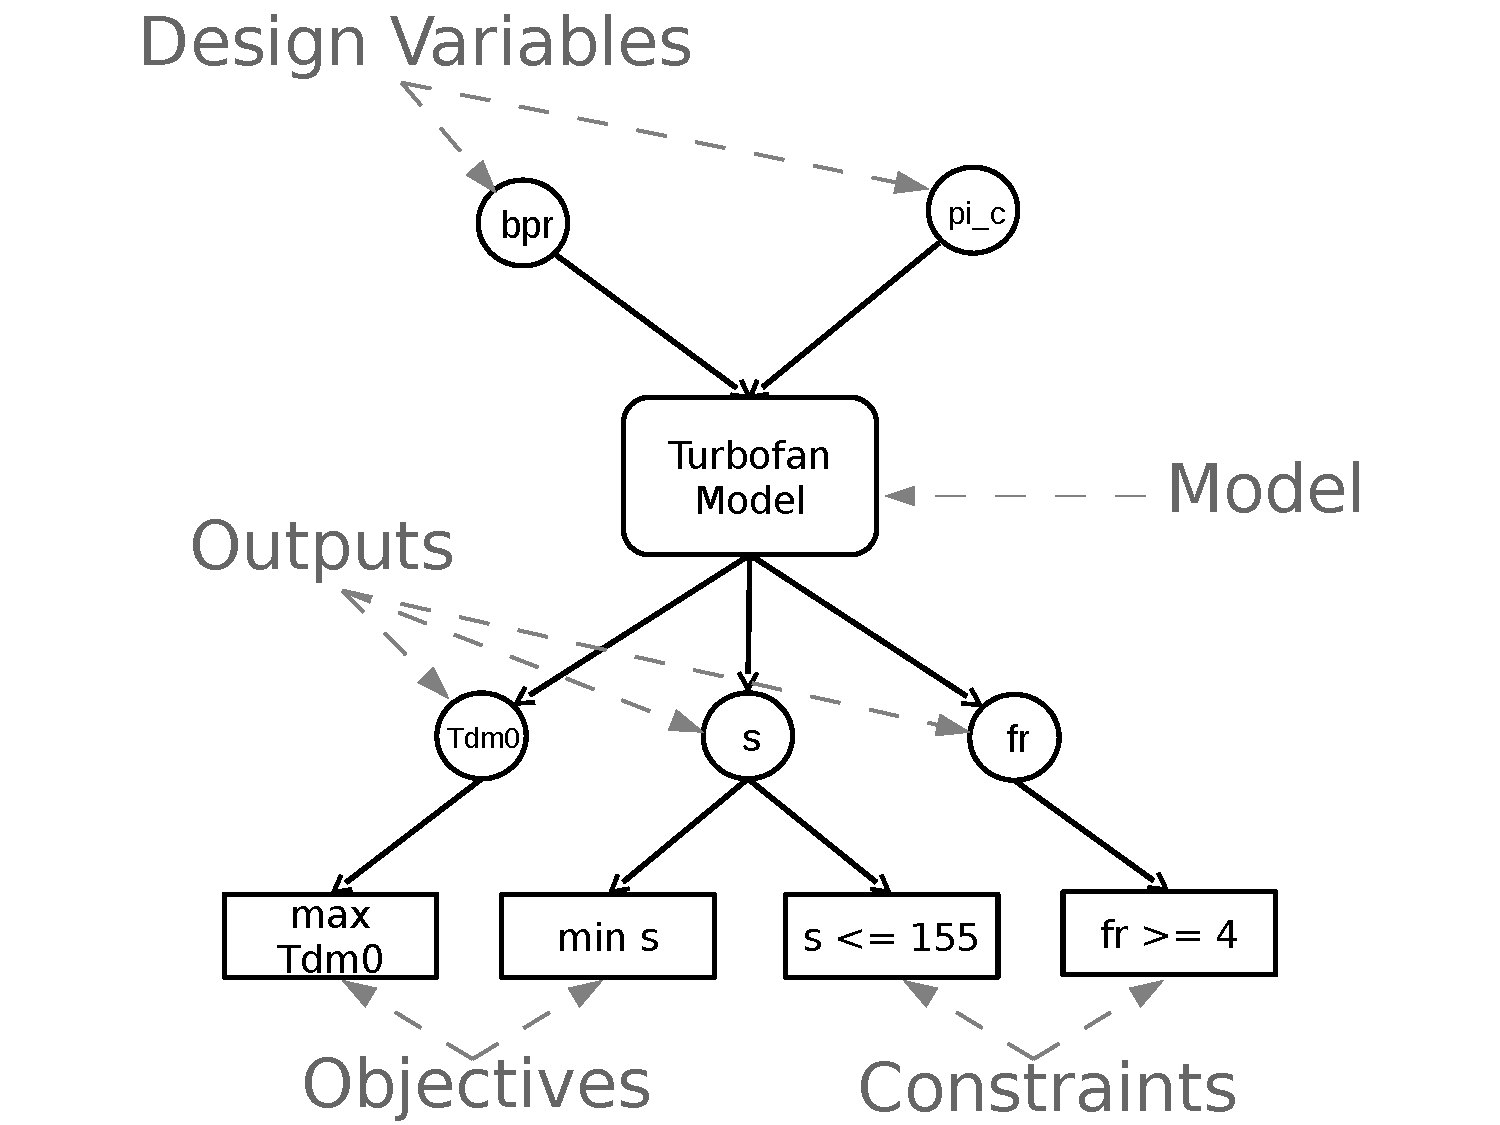
\includegraphics[width=\textwidth]{testcases-Turbofan-annoted}
			\caption{corresponding entities graph.}\label{turbofan:graph}
	\end{subfigure}
\caption{Turbofan problem.}
\label{turbofan}

\end{figure}

Let us now see in more details the roles of each of these fives entities: \emph{model}, \emph{variable}, \emph{output}, \emph{constraint} and \emph{objective}.

\subsection{Models}

In the most general case, a \emph{model} can be seen as a black box which takes input values (which can be \emph{design variables} or \emph{outputs}) and produces some output values. A \emph{model} represents a technical knowledge of the relations between different parts of a problem and can be as simple as a linear function or a much more complex algorithm requiring several hours of calculation. Often some properties are known (or can be deduced) about a model and specialized optimization techniques can exploit this information. It is important to understand that what exactly is a \enquote{model} is quite an arbitrary choice, based on the application domain of the problem. Depending on the goals and needs, a same problem will be divided into models of different granularities and scopes. A model can represent a simple calculus step as well as an entire discipline.

In our Turbofan example on \figurename{} \ref{turbofan}, the $Turbofan$ function is a \emph{model} entity which calculates the three outputs using the values of $bpr$ and $pi\_c$ (marked $\pi_c$ in the equations of the model). The equations contained in the model itself are described on algorithm \ref{algo_turbofan}.

\begin{algorithm}
\caption{Turbofan Model}
\label{algo_turbofan}

	\KwIn{$bpr$, $\pi_c$}
	\;
	\tcp{constants}
	$\gamma =1.4$\;
	$cp = 1004.5$\;
	$hfuel = 42.8 \times 1e+06$\;
	$\alpha_{thrust} 	= 1.0$\;
	$t0 		= 216.7$\;
	$m0 		= 0.83$\;
	$\eta_c 		= 0.9$\;
	$\eta_f 		= 0.9$\;
	$ttburn 		= 1560.0$\;
	$\pi_f 		= 1.7$\;
	\;
	$r	\leftarrow (\gamma-1) \times \dfrac{cp}{\gamma}$\;
	$a0	\leftarrow \sqrt{\gamma \times r \times t0}$\;
	$u0	\leftarrow m0 \times a0$\;
	$\tau_r	\leftarrow 1+\dfrac{\gamma-1}{2} \times m0^2$\;
	$\tau_\lambda \leftarrow \dfrac{ttburn}{t0}$\;
	$\tau_c	\leftarrow \pi_c^{\dfrac{\gamma-1}{\eta_c \times \gamma}}$\;
	$\tau_f	\leftarrow \pi_f^{\dfrac{\gamma-1}{\eta_f \times \gamma}}$\;
	$\tau_t	\leftarrow 1-\dfrac{tau_r}{tau_\lambda} \times ((\tau_c-1)+bpr \times (\tau_f-1))$\;

	$UeU0	\leftarrow \sqrt{\dfrac{\tau_r \times tau_c \times \tau_t-1}{\tau_r-1} \times \dfrac{\lambda}{\tau_r \times \tau_c}}$\;
	$UfU0	\leftarrow \sqrt{\dfrac{\tau_r \times \tau_f-1}{\tau_r-1}}$\;
	\;
	\tcp{outputs computation}	
	$Tdm0	\leftarrow u0 \times \dfrac{1}{(1+bpr)} \times (UeU0-1)+\dfrac{bpr}{1+bpr} \times (UfU0-1)) \times \alpha_{thrust}$;
	%$f	\leftarrow \dfrac{cp \times t0 \times (\tau_\lambda-\tau_r \times \tau_c)}{hfuel}$\;
	$s	\leftarrow \dfrac{f}{(1+bpr) \times Tdm0} \times 10e+06$\;
	%$rend_p \leftarrow 2 \times \dfrac{ UeU0-1+bpr \times (UfU0-1)}{UeU0^2-1+bpr \times (UfU0^2-1)}$\;
	$fr	\leftarrow \dfrac{UeU0-1}{UfU0-1}$\;

\end{algorithm}

\subsection{Design Variables}

These are the inputs of the problem and can be adjusted freely (within their defined boundaries). The goal of the optimization process is to find the set(s) of values for these variables that maximize the objectives while satisfying the constraints. A \emph{design variables} can be used by \emph{models} to calculate their output values and by \emph{constraints} and \emph{objectives} to calculate their current value. A \emph{design variable} can be shared among several \emph{models}, \emph{objectives} and \emph{constraints}.

Keeping with our example on \figurename{} \ref{turbofan}, the bypass ratio $bpr$ and the compressor pressure ratio $pi\_c$ are the two \emph{design variables} of our optimization problem.

\subsection{Outputs}

These values are produced by a \emph{model}, and consequently cannot be changed freely.
As for the \emph{design variables}, the \emph{outputs} can be used by \emph{models} to calculate their output values and by and by \emph{constraints} and \emph{objectives} to calculate their current value.

In our example on \figurename{} \ref{turbofan}, the thrust $Tdm0$, the fuel consumption $s$ and the thrust ratio $fr$ are \emph{outputs} produced by the $Turbofan$ model.

\subsection{Constraints}

They are strict restrictions on some parts of the problem, represented as functional constraints defined by equalities and/or inequalities. They can be the expression of a physical limitation, or a requirement concerning the problem.

Regarding the Turbofan on \figurename{} \ref{turbofan}, the two \emph{constraints} are $s <= 155$ and $fr >=4$.

\subsection{Objectives}

The goals to be optimized. In the general case, different \emph{objectives} are often contradictory.

The two \emph{objectives} of the Turbofan problems on \figurename{} \ref{turbofan} are to maximize th thrust $Tdm0$ and to minimize the fuel consumption $s$.

\emph{Constraints} and \emph{objectives} are usually regrouped under the more general term of optimization criteria. 

\paragraph*{}
An interesting and important point is that both models, constraints and objectives involve computation. Often the most heavyweight calculus is encapsulated inside a model and the calculi concerning criteria tend to be simple equations, but this is neither an absolute requirement nor a discriminating characteristic.

Using this decomposition, the optimization problem can then be represented as a graph $ G = (V, E)$, where the vertices set $V$ is a tuple $\langle \mathcal{V}_d, \mathcal{V}_o, \mathcal{M}, \mathcal{O}, \mathcal{C}\rangle$ (denoting respectively the sets of design variables, outputs, models, objectives and constraints of the problem), and $E$ is the set of relations between the entities. It can be noted that the graph is bipartite regarding the two sets $(\mathcal{V}_d \cup \mathcal{V}_o)$ and $(\mathcal{M} \cup \mathcal{O} \cup \mathcal{C})$, as design and output variables can only be connected to models, objectives or constraints, which can themselves only be connected to design or output variables.
Using our Turbofan example, the tuple $\langle \mathcal{V}_d, \mathcal{V}_o, \mathcal{M}, \mathcal{O}, \mathcal{C}\rangle$ of the graph representing this problem is defined as:
\begin{align*}
	\mathcal{V}_d &= \{bpr, pi_c\}, \\
	\mathcal{V}_o &= \{Tdm0, s, fr\},\\
	\mathcal{M} &= \{Turbofan\_Model\},\\
	\mathcal{O} &= \{\text{max }Tdm0, \text{min }s\},\\
	\mathcal{C} &= \{s <= 155, fr >= 4\}.
\end{align*}

The NDMO modeling aims to provide the most complete and natural representation of the problem. This modeling preserves the relations between the domain entities and is completely independent of the solving process. The distinct entities that are extracted from the analytical formulation of the problem do not come from an arbitrary decision but are inherent to the problem formulation. On the other hand, all the relationships present between these entities are preserved without any simplification regarding the initial complexity of the problem.

\section{From an Optimization Problem to a Multi-Agent System}

Based on the NDMO modeling in section \ref{modeling}, we propose a MAS where each domain entity is associated with an agent. Thus the MAS is the representation of the problem to be solved, with the relationships between agents reflecting the natural structure of the problem. It is worth underlining the fact that this transformation (\textit{i.e.} the agentification) is completely automatic, as it is fully derived from the expression of the problem.

The solving process ---constituted by the collective behavior of the agents--- basically relies on change-value requests sent by the criteria agents, resulting in cooperatively decided adjustments done by the \emph{design variables}. These adjustments lead to new values computed by the models, resulting on the satisfaction or dissatisfaction of the criteria agents. 
In the same way we presented the different elements of NDMO, we now detail the behaviors of our five agent types: \emph{model}, \emph{variable}, \emph{output}, \emph{constraint} and \emph{objective} agents.

\subsection{Model Agent}

A \emph{model agent} takes charge of a model of the problem. It interacts with the agents handling its inputs (which can be \emph{variable} or \emph{output agents}) and the \emph{output agents} handling its outputs. Its individual goal is to maintain the consistency between its inputs and its outputs. To this end, when it receives a message from one of its inputs informing it of a value change, a \emph{model agent} recalculates the outputs values of its model and informs its \emph{output agents} of their new value (as seen on \figurename{} \ref{agent_behav_model:inf}). On the other part, when a \emph{model agent} receives a request from one of its \emph{output agents} it translates and transmits the request to its inputs (as seen on \figurename{} \ref{agent_behav_model:req}). 

\begin{figure}
\centering
\begin{subfigure}{0.35\textwidth}
		\centering
		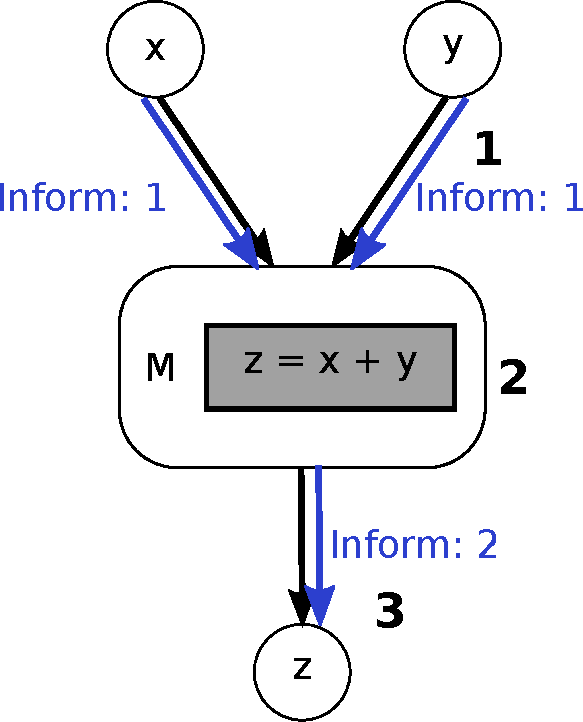
\includegraphics[width=\textwidth]{agent_behav_model_inform}
		\caption{Inform handling:\\1. receive informs.\\2. recalculate outputs.\\3. propagate informs.}\label{agent_behav_model:inf}
\end{subfigure}
\qquad
\begin{subfigure}{0.35\textwidth}
		\centering
		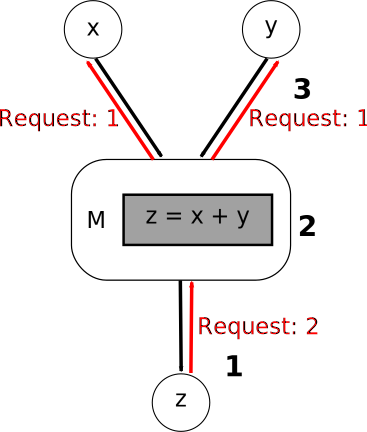
\includegraphics[width=\textwidth]{agent_behav_model_request}
		\caption{Request handling:\\1. receive request.\\2. estimate inputs changes.\\3. propagate request.}\label{agent_behav_model:req}
\end{subfigure}
\caption{Model agent behavior.}\label{agent_behav_model}
\end{figure}

To find the input values corresponding to a specific desired output value, the \emph{model agent} uses an external optimizer. This optimizer is provided by the engineer based on domain-dependent expert knowledge regarding the structure of the model itself.
It is important to underline that the optimizer is used only to solve the local problem of the \emph{model agent}, and is not used to solve the optimization problem globally.

\subsection{Variable Agent}

This agent represents a \emph{design variable} of the problem. Its individual goal is to find a value which is the best equilibrium among all the requests it receives (from models and criteria for which it is an input). The agents using the variable as input can send requests asking it to change its value. When changing value, the agent informs all the related agents of its new value. This behavior is shown on \figurename{} \ref{agent_behav_variable}. 

\begin{figure}
\centering
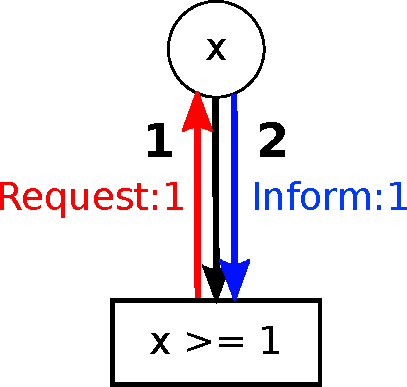
\includegraphics[width=0.3\textwidth]{agent_behav_variable}
\caption{Variable agent behavior:\\1. receive request.\\2. answer with inform.}\label{agent_behav_variable}
\end{figure}

\subsection{Output Agent}
The \emph{output agent} takes charge of an output of a model. \emph{Output agent} and \emph{variable agents} have similar roles, except that \emph{output agents} cannot directly change their value. Instead they send a request to the \emph{model agent} they depend on. In this regard, the \emph{output agent} act as a filter for its \emph{model agent}, selecting among the different requests the ones it transmits. This behavior is summarized on \figurename{} \ref{agent_behav_output}.

\begin{figure}
\centering
\begin{subfigure}{0.25\textwidth}
		\centering
		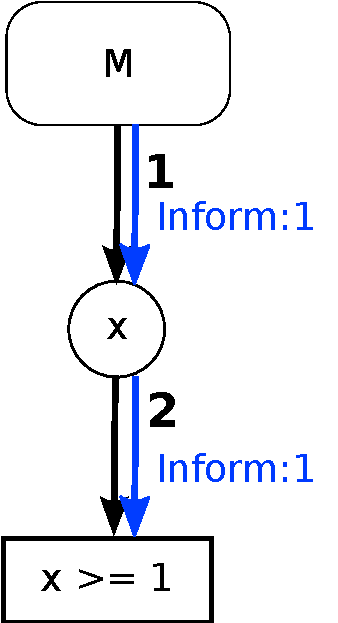
\includegraphics[width=\textwidth]{agent_behav_output_inform}
		\caption{Inform handling:\\1. receive inform.\\2. propagate inform.}\label{agent_behav_output:inf}
\end{subfigure}
\qquad
\begin{subfigure}{0.25\textwidth}
		\centering
		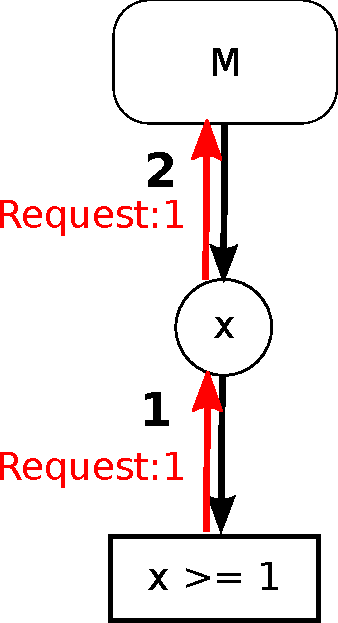
\includegraphics[width=\textwidth]{agent_behav_output_request}
		\caption{Request handling:\\1. receive request.\\2. propagate request.}\label{agent_behav_output:req}
\end{subfigure}
\caption{Output agent behavior.}\label{agent_behav_output}
\end{figure}

%As we will see in the next section, the \emph{output agent} is distinct from the \emph{variable agent} in the way that it can be involved in cycles. A cycle is a situation of interdependent models (that is, models which depend of each other to calculate their outputs).

\subsection{Constraint Agent}
 \emph{The constraint agent} has the responsibility for handling a constraint of the problem. When receiving a message from one of its inputs, the agent recalculates its constraint and checks its satisfaction. If the constraint is not satisfied, the agent sends \emph{change value} requests to its inputs. The behavior of the agent is illustrated on \figurename{} \ref{agent_behav_constraint}.
 
\begin{figure}
\centering
\begin{subfigure}{0.3\textwidth}
	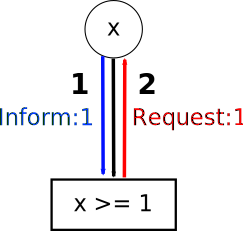
\includegraphics[width=\textwidth]{agent_behav_constraint}
	\caption{Constraint agent behavior:\\1. receive inform.\\2. answer with request.}\label{agent_behav_constraint}
\end{subfigure}
\qquad
\begin{subfigure}{0.3\textwidth}
	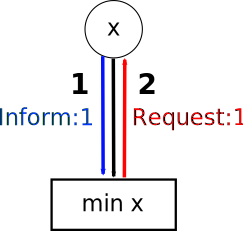
\includegraphics[width=\textwidth]{agent_behav_objective}
	\caption{Objective agent behavior:\\1. receive inform.\\2. answer with request.}\label{agent_behav_objective}
\end{subfigure}
\caption{Constraint and objective agents behavior.}\label{agent_behav_constraint_and_objective}
\end{figure}

It should be noted that, to estimate the input values required to satisfy the constraint on its computed value, this agent employs the same technique as the \emph{model agent} (\textit{i.e.} an external optimizer).

\subsection{Objective Agent}
The \emph{objective agent} is in charge of an objective of the problem. This agent sends requests to its inputs aiming to improve its objective, and recalculates the objective when receiving \emph{value changed} messages from its inputs.

This agent uses an external optimizer to estimate input values that would improve the objective, in the same way than the \emph{model} and \emph{constraint agents}.

\begin{figure}
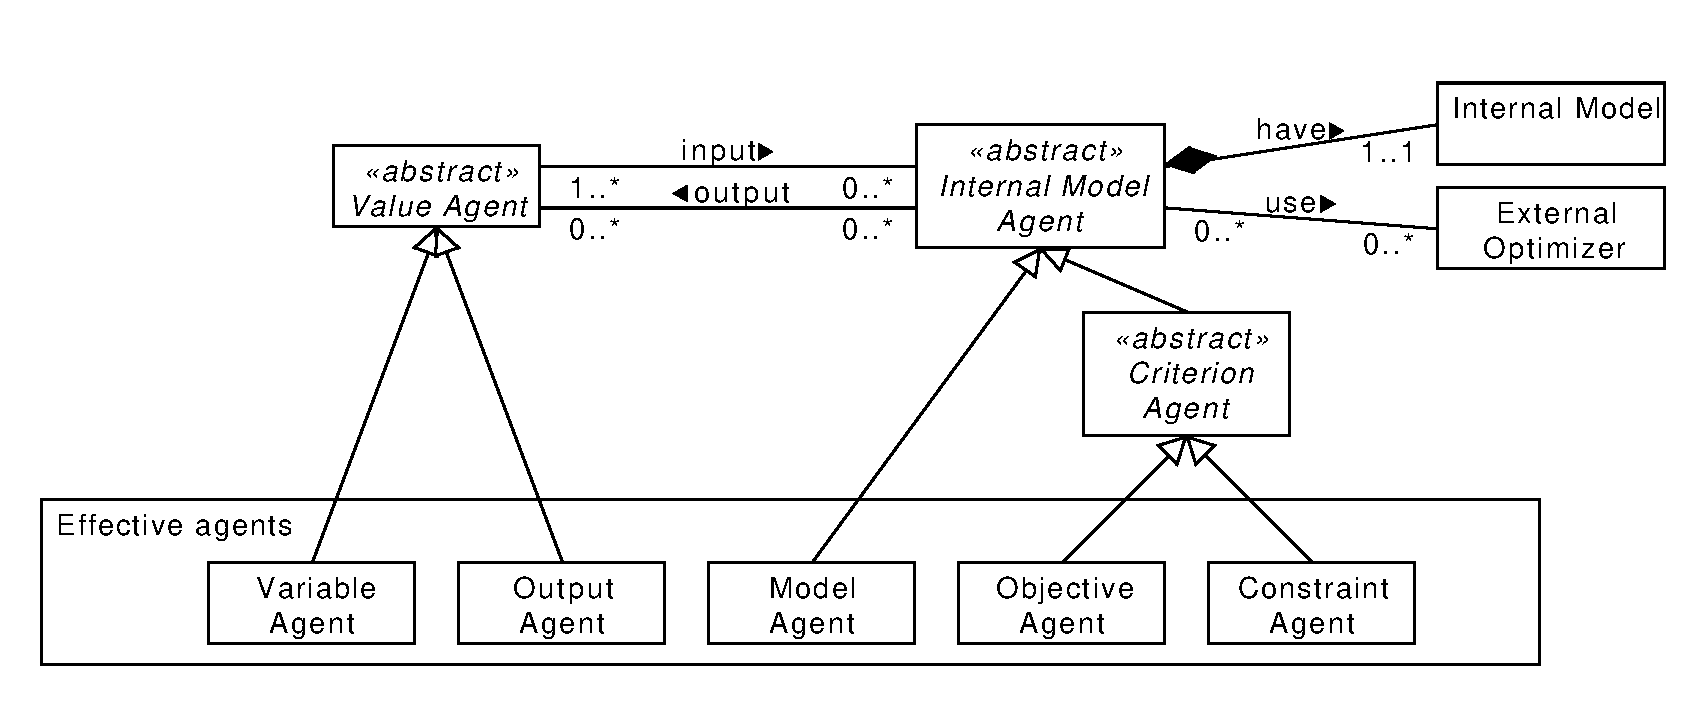
\includegraphics[width=0.9\textwidth]{agent_class_diag}
\caption{MAS class diagram.}\label{MAS_class_diagram}
\end{figure}

\paragraph*{}
This agent modeling is the most direct and inclusive, considering every element of the problem as an autonomous agent. On \figurename{} \ref{MAS_class_diagram} we represent a class diagram of the agents, which is a slightly modified version of the domain class diagram of \figurename{} \ref{class_diag}. This modified class diagram puts more clearly in light what are the effective agents and how the agents are related with each others by input/output relationships. The bipartite nature of the graph in regard of \emph{value agents} and \emph{internal model agents} is clearly apparent. Two additional, non-agent entities, the \emph{internal model} and the \emph{external optimizer} also made an appearance. The respective roles of these two entities will be detailed in the next chapters.

\chapter{Agents Behavior}\label{agent_behav_chap}

We will now discuss the behavior of the five agent types identified in the previous chapter. The functioning of the system can be divided into two main tasks: problem simulation and collective solving.

Problem simulation can be seen as the equivalent of the analysis of classical MDO methods. The agents behavioral rules related to problem simulation concern the propagation of the values of design variables to the models and criteria. For this part, the agents will exchange \emph{inform} messages that contain calculated values. The \enquote{messages flow} is top-down: the initial inform messages will be emitted by the variable agents and will be propagated down to the criteria agents. An illustration of the simulation messages flow is shown on \figurename{} \ref{messages_flow:inf}.

Collective solving concerns the optimization of the problem. The agent behavioral rules related to collective solving are about satisfying the constraints while improving the objectives. For this part, the agents will exchange \emph{request} messages which contain desired variations of values. The \enquote{messages flow} is bottom-up: the initial request messages will be emitted by the criteria agents and propagated up to variable agents. An illustration of the solving messages flow is shown on \figurename{} \ref{messages_flow:req}.

\begin{figure}[h]
	\begin{subfigure}[b]{0.4\textwidth}
		\centering
		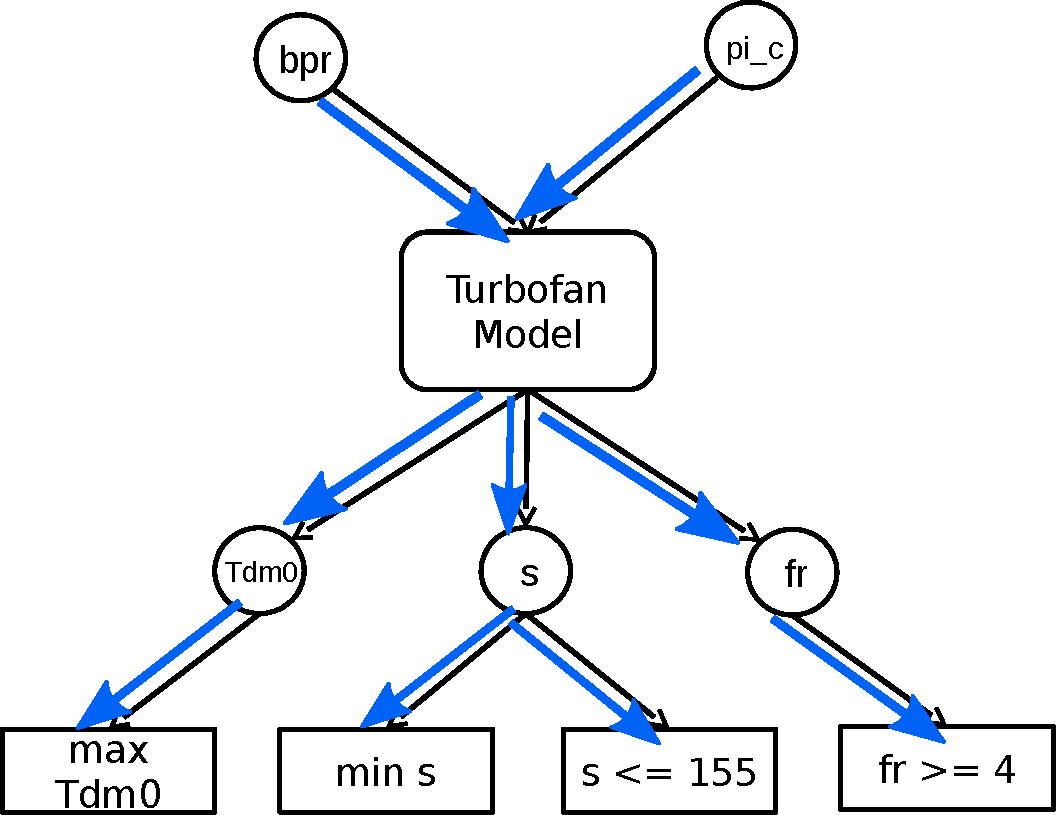
\includegraphics[width=\textwidth]{testcases-Turbofan-informs}
		\caption{Informs flow for simulation.}\label{messages_flow:inf}
	\end{subfigure}
	\hfill
	\begin{subfigure}[b]{0.4\textwidth}
		\centering
		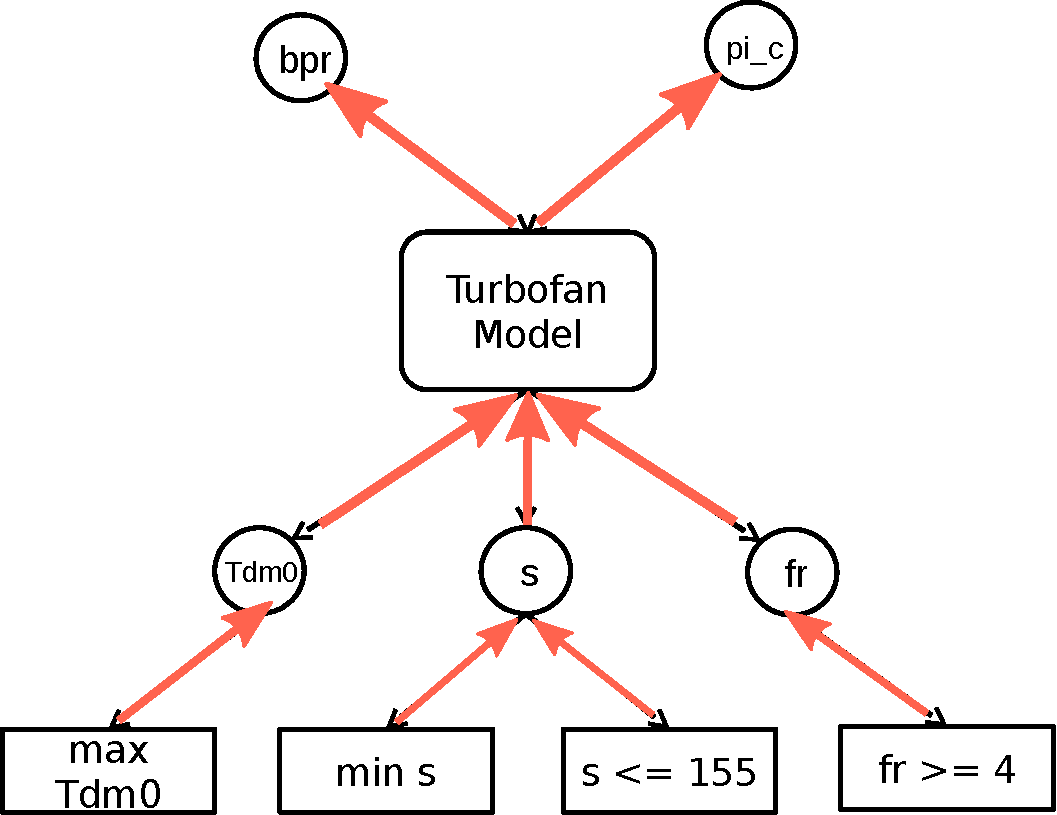
\includegraphics[width=\textwidth]{testcases-Turbofan-requests}
		\caption{Requests flow for solving.}\label{messages_flow:req}
	\end{subfigure}

	%new line
	\centering
	 \begin{subfigure}[b]{0.4\textwidth}
		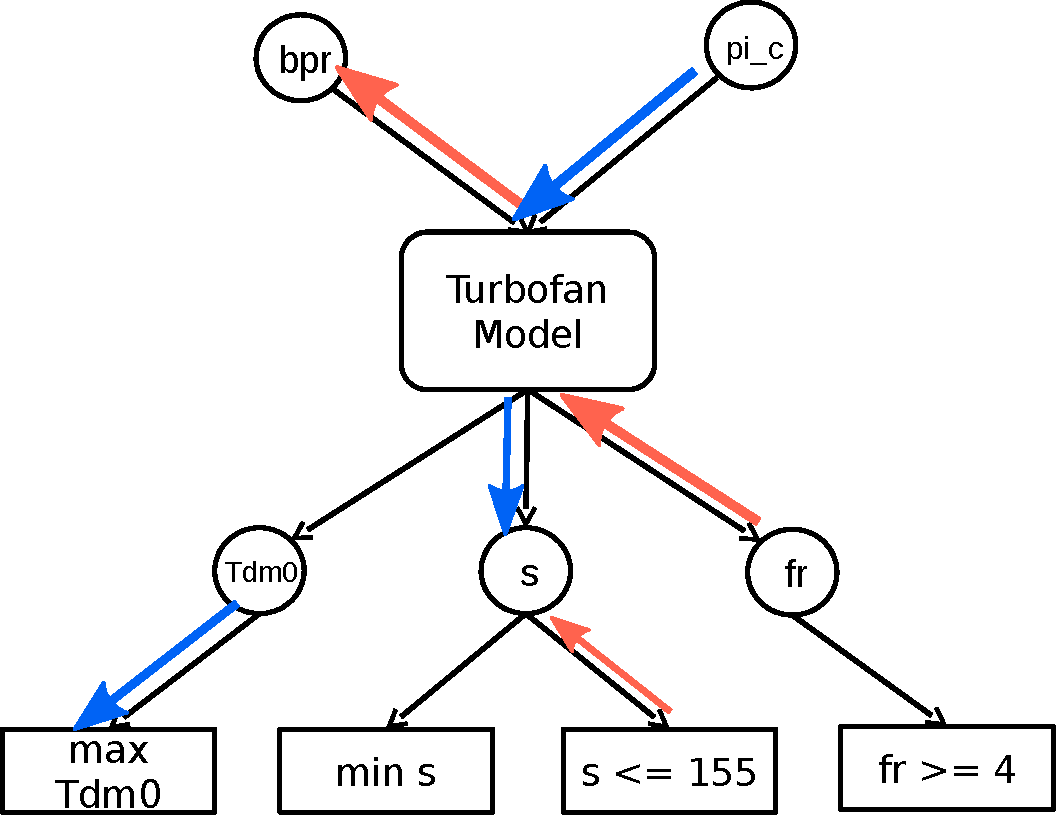
\includegraphics[width=\textwidth]{testcases-Turbofan-informs_requests}
		\caption{Effective messages flow.}\label{messages_flow:eff}
	\end{subfigure}
	
	\caption{Messages flow for simulation and solving.}
	\label{messages_flow}

\end{figure}

The agents behaviors regarding these two parts can be studied independently, we will thus present them separately. It is however important to remember that these two parts are executed simultaneously. At runtime the agents will simulate the problem and solve it in parallel. Moreover, the different parts of the system will not necessarily work in a synchronous fashion. The effective messages flow of the system will more probably be akin to the \figurename{} \ref{messages_flow:eff}.

\section{Problem Simulation}

In this section we will present the agents behaviors related to the simulation of the problem. Regarding this part, the main concern of the agents is to ensure consistency between the values of the design variables and the produced outputs. To this end, the agents will propagate \emph{Inform} messages through the system.

An inform message carries a new value $v$. The exact semantic of this information slightly changes depending on which agents are involved:

\begin{itemize}
\item If the message is sent from a value agent (variable or output) to a model or criterion agent, it indicates to the receiving agent that the sending agent has changed of value.

\item If the message is sent from a model agent to an output agent, it indicates to the receiving agent that the model has calculated its new value.
\end{itemize}

In practice this distinction is not fundamentally important to understand the functioning of the system.

As stated in section \ref{modeling}, models, constraints and objectives involve a specific calculation operation. For example the constraint $x -y \geq 0$ implies the very basic calculation $x - y$. We regroup these operations under the term \emph{internal models}. As we said, no specific hypothesis is done concerning the nature of an internal model and, more importantly, no distinction is done regarding the internal model used by a model agent and the one used by an objective or a constraint agent.\\
While in some cases specific informations can be known regarding the nature of an internal model, in the most general case these internal models can be seen as black boxes and are handled as such by the agents.

\subsection{Variable Agent}

Regarding problem simulation, the role of the variable agent is to ensure that the agents to which it is connected know its current value.
A variable agent has to send new Inform messages when:
\begin{compactitem}
\item new agents are connected to it (typically at the creation of the system).
\item it decides to change its value based on received requests (see \ref{variable_agent_solving}).
\item the designer changed its value.
\end{compactitem}

The behavior of the variable agent is summarized in algorithm \ref{algo_simulating_variable}. First of all the variable checks if it changed its value (typically as the consequence of receiving requests during the solving phase). If it is the case it sends its new value to its contacts. It then checks if new agents have requested to be added to its contacts. If it is the case, it adds them and sends them its current value, whether its value changed or not, in order for the new contacts to be informed of the current value of the variable.

\begin{algorithm}
\caption{Problem Simulation -- Variable Agent Behavior}
\label{algo_simulating_variable}

	$C \leftarrow$ previously connected agents\;
	$C'\leftarrow$ newly connected agents\;
		
	$v \leftarrow$ previous value\;
	$v'\leftarrow$ new value\;
	
	\tcp{notify contacts of value change}
	\If{$v \neq v'$}{
		$v \leftarrow v'$\;
		\ForEach{agent $a \in C$}{
			send($a$, new Inform($v$))\;
		}
	}
	
	\tcp{send its value to new contacts}
	\tcp{even if it did not change}
	\If{$C' \neq \emptyset$}{
		\ForEach{agent $a \in C'$}{
			send($a$, new Inform($v$))\;
		}
		$C \leftarrow C \bigcup C'$\tcp{memorize new connected agents}
	}
	
\end{algorithm}

\subsection{Model Agent}\label{simulation_model}

A model agent must maintain consistency between its inputs and outputs. That is, it must ensure that the agents handling its output variables are informed of their new values when the inputs changes. When receiving an Inform message from one of the agents controlling its inputs, the model agent reevaluates its internal model, taking the new value into account. Using the new values produced by the internal model, the model agent then sends Inform messages to the agents responsible of its outputs.

All outputs of a model agent are not necessarily associated with an output agent. For example, if the designer is not interested by the value represented by one of the outputs, he is not required to represent it by an agent. In this case the model agent will silently calculate the new value of the output at the same time than the others, but will not propagate it\footnote{Remember that the internal model of the agent is a black box, consequently the agent cannot choose to evaluate it partially. If the evaluation of the output could has been done independently from the others, it may be preferable to create two separate models}.

However, as the problem is dynamic, the designer can decide at any time to connect a new output agent to a previously unconnected output. In this case, the model agent must send to the output agent the last value it calculated for this output.

The behavior of the model agent is summarized in algorithm \ref{algo_simulating_model}.

\begin{algorithm}
\caption{Problem Simulation -- Model Agent Behavior}
\label{algo_simulating_model}

	$C \leftarrow$ previously connected output agents\;
	$C'\leftarrow$ newly connected output agents\;
	$\{v_o\} \leftarrow$ previous output values\;
	$\{v_i\} \leftarrow$ new input values\;

	\If{$\{v_i\} \neq \emptyset$}{
		\tcp{use internal model to recalculate outputs}
		$\{v_o\}\leftarrow Internal\_Model(\{v_i\})$\;
		\ForEach{agent $a_o \in C$}{
			\tcp{inform output agents of their new value}
			send($a_o$, new Inform($v_o$))\;
		}
	}
	
	\tcp{send their values to new outputs}
	\tcp{even if they did not change}
	\If{$C' \neq \emptyset$}{
		\ForEach{agent $a_o \in C'$}{
			send($a_o$, new Inform($v_o$))\;
		}
		$C \leftarrow C \bigcup C'$\tcp{memorize new outputs agents}
	}
	
\end{algorithm}

\subsection{Output Agent}

For the problem simulation, the output agent has a very similar role to the variable agent. It tries to ensure that the agents to which it is connected know its current value. It has to change new inform messages when:
\begin{compactitem}
\item new agents are connected to it.
\item it receives an inform message from its model agent, indicating it its new value.
\end{compactitem}

Unlike the variable agent, the output agent value should not be directly changed by the designer, as it represents a non-free variable.

The behavior of the output agent is summarized in algorithm \ref{algo_simulating_output}.

\begin{algorithm}
\caption{Problem Simulation -- Output Agent Behavior}
\label{algo_simulating_output}

	$C \leftarrow$ previously connected output agents\;
	$C'\leftarrow$ newly connected output agents\;
		
	$v \leftarrow$ previous value\;
	$v'\leftarrow$ new value\;
	
	\tcp{notify output contacts of value change}
	\If{$v \neq v'$}{
		$v \leftarrow v'$\;
		\ForEach{agent $a \in C$}{
			send($a$, new Inform($v$))\;
		}
	}
	
	\tcp{send its value to new output contacts,}
	\tcp{even if it did not change}
	\If{$C' \neq \emptyset$}{
		\ForEach{agent $a \in C'$}{
			send($a$, new Inform($v$))\;
		}
		$C \leftarrow C \bigcup C'$\tcp{memorize new connected agents}
	}
	
\end{algorithm}

At runtime, the designer can interact with the MAS. Among the possible interactions, the designer can remove the model calculating an output. In this case the output agent would become a variable agent and change its behavior accordingly. The inverse transformation is also possible, a variable agent could suddenly be \enquote{plugged} in an output of a model and would become an output agent.

\subsection{Constraint/Objective Agent}

In regard to problem simulation, constraint and objective agents only role is to update their value based on the Inform they receive from their inputs.

Their behavior is summarized in algorithm \ref{algo_simulating_criterion}.

\begin{algorithm}
\caption{Problem Simulation -- Constraint/Objective Agent Behavior}
\label{algo_simulating_criterion}

	$\{v_i\} \leftarrow$ new input values\;
			
	\If{$\{v_i\} \neq \emptyset$}{
		\tcp{use internal model to recalculate outputs}
		$\{v'_o\}\leftarrow Internal\_Model(\{v_i\})$
	}

\end{algorithm}

\section{Collective Solving}\label{collective_solv}

During solving, the criteria agents try to improve their local goals. That is, the constraint agents try to keep their constraint satisfied, while the objective agents try to improve their objective. To this end, they send \emph{Request} messages to the agents controlling their inputs, asking them to change value. The others agents have to propagate these requests toward the variable agents in the most adequate way.

However a specific difficulty arises. As explained in the previous section, model, constraint and objective agents manipulate the underlying equations (or algorithms, or responses surfaces \emph{etc.}) of the problem through internal models, which are in most cases black boxes. In this case, how can constraint agents know which values to ask to satisfy their constraint? How can objective agents know the values that improve their objective? How can model agents know which values for their inputs could produce the values required by their outputs?\\
For the internal model agents to be able to work, the designer must supply them with an \emph{external optimizer}. The role of this optimizer is the following: if we see an internal model as a function\footnote{Calling an internal model a function is a simplification. Since it is a black box it may have an internal state. Consequently the same inputs may not always produce the same outputs} providing an output $O$ from a set of input $I$, what we need is to be able to estimate the inverse function, providing the values of $I$ corresponding to a specific $O$. This specific problem can easily be expressed as a classical optimization problem in itself, which can be solved by classical optimization methods. As the agents manipulate black boxes, it is (nearly\footnote{We will see in section \ref{model_agent_solving} how the agents can extract enough information at runtime to provide their own basic optimizer}) impossible for them to do this estimation by themselves. The designer, which has a more advanced knowledge of the internal models, can provide an adequate optimization method for each of them. In the most general case it can be assumed that each agent in charge of an internal model uses its own specific optimizer. However in practice several instances of the same optimizer can be used by different agents, if the designer deems that their models present sufficient similar characteristics for the optimization method to be efficient for each of them. An example of use of an external optimizer by a model agent can be seen on \figurename{} \ref{optim_use}.

\begin{figure}
	\centering
	\begin{subfigure}[b]{0.32\textwidth}
		\centering
		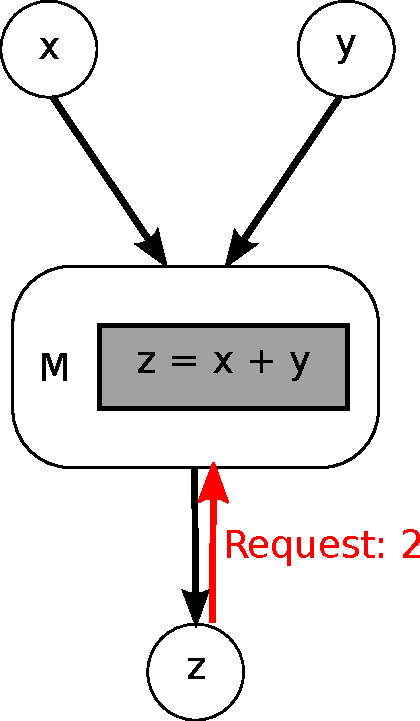
\includegraphics[height=5cm]{optim_use_1}
		\caption{The model agent receives a request.}\label{optim_use:1}
	\end{subfigure}
	\hfill
	\begin{subfigure}[b]{0.32\textwidth}
		\centering
		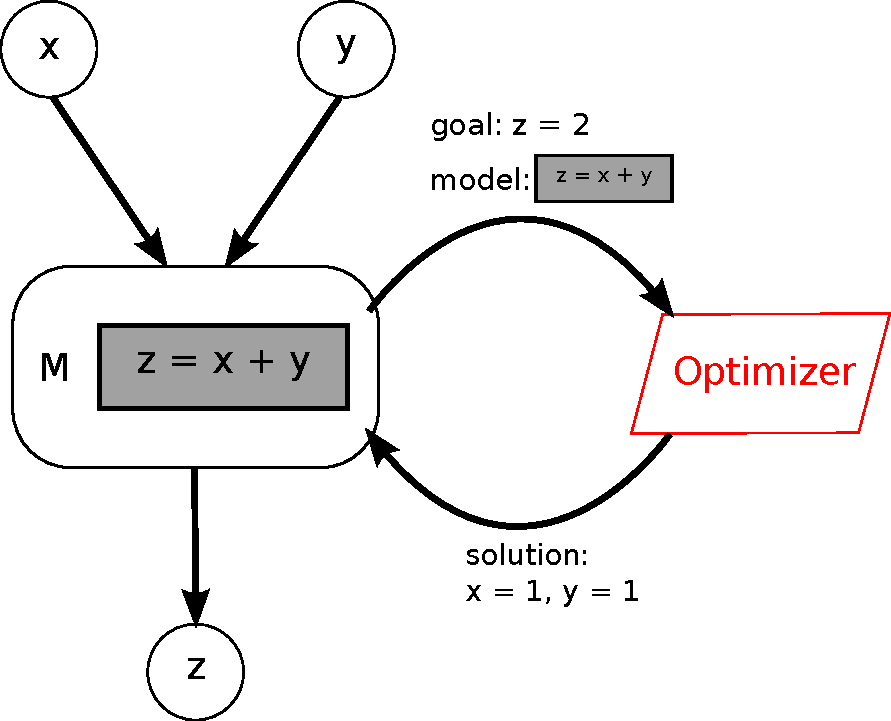
\includegraphics[height=5cm]{optim_use_2}
		\caption{The model agent resolves the request using an external optimizer.}\label{optim_use:2}
	\end{subfigure}
	\hfill
	\begin{subfigure}[b]{0.32\textwidth}
		\centering
		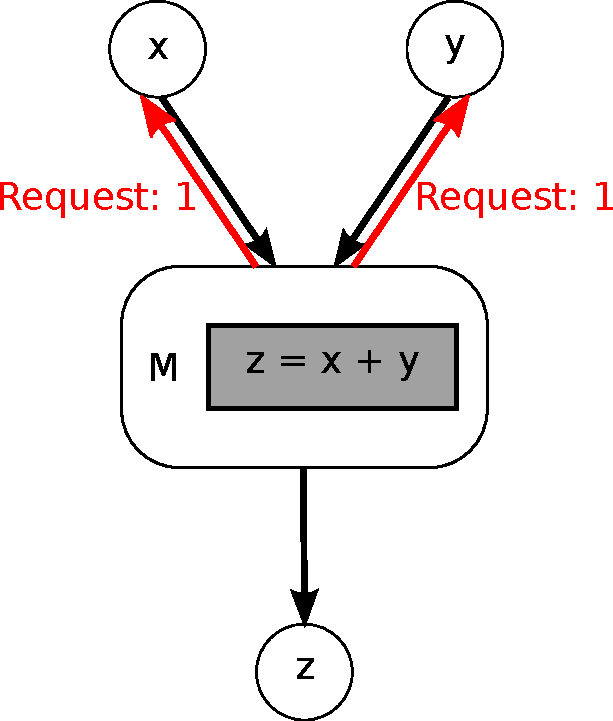
\includegraphics[height=5cm]{optim_use_3}
		\caption{The model agent transmits the new requests to its inputs.}\label{optim_use:3}
	\end{subfigure}
	\caption{Use of an external optimizer.}\label{optim_use}
\end{figure}

As a remark, finding the inputs corresponding to a desired value is not directly an optimization problem, but is trivial to translate into one. For example, the problem can be formulated as finding $I$ that minimizes $(f(I) - O)^2$. Alternatively, the objective-function can be replaced by a constraint such as $f(I) = O$. We do not impose a specific transformation method, letting the expert which implements the optimizer chooses which transformation is the most efficient in regard to the specificities of the optimization method.

With this specificity in mind, let us now examine the behavior of the different agent types in the context of collective solving.

\subsection{Variable Agent}\label{variable_agent_solving}

During solving, a variable agent is susceptible to receive change requests from other agents. When a variable agent receives a change request, it tries to change its own value in order to accommodate the requester while taking into account the previous demands of the rest of its neighbors. To this end, the variable agent uses an exploration strategy based on \emph{Adaptive Value Tracker} (AVT) \cite{Lemouzy_2011}. The AVT is an adaptation of dichotomous search for dynamic values. The idea is to change value according to the direction which is requested and the direction of the past requests. While the value varies in the same direction, the variation delta is increased so the value varies more and more. As soon as the requested variation changes, it means that the variable went past the good value, so the variation delta is reduced.
This capability to take into account a changing solution allows the variable agent to continuously search for an unknown dynamic target value. This capability is required for the system to be able to adapt to changes made by the engineer during the solving process.

The algorithm of the AVT is the following. Given the following variables:
\begin{itemize}
\item $v_t \in [v_{min};v_{max}]$ the current value of the AVT.
\item $\Delta_t \in [\Delta_{min};\Delta_{max}]$ the last variation of $v_t$.
\item $\lambda_i$ the increase coefficient of the AVT ($\lambda_i > 1$).
\item $\lambda_d$ the decrease coefficient of the AVT ($0 < \lambda_d < 1$).
\end{itemize}

When receiving a new adjustment feedback $Fb_t \in \{\uparrow ; \downarrow ; \sim\}$ (corresponding respectively to \enquote{increase current value}, \enquote{decrease current value} and \enquote{keep current value}), a new value $v_{t+1}$ is calculated using \tablename{} \ref{tab:avt}. 

\begin{table}[h]
\centering
\begin{tabular}{ c  c  c  c  c  }
\toprule
& &\multicolumn{3}{c}{$Fb_t$} \\
  &             & $\uparrow$ & $\downarrow$ & $\sim$ \\ \toprule
  & \multirow{2}*{$\uparrow$}  &  $\Delta_t = \Delta_{t-1} \times \lambda_i$  & $\Delta_t = \Delta_{t-1} \times \lambda_d$  &   $\Delta_t = \Delta_{t-1} \times \lambda_d$      \\ 
    &   &  $v_{t+1} = v_t + \Delta_t$  &   $v_{t+1} = v_t - \Delta_t$  &  $v_{t+1} = v_t $       \\ \cmidrule{2-5}
\multirow{2}*{$Fb_{t-1}$}  & \multirow{2}*{$\downarrow$}  &  $\Delta_t = \Delta_{t-1} \times \lambda_d$  & $\Delta_t = \Delta_{t-1} \times \lambda_i$  &   $\Delta_t = \Delta_{t-1} \times \lambda_d$      \\ 
  &   &  $v_{t+1} = v_t + \Delta_t$  &   $v_{t+1} = v_t - \Delta_t$  &  $v_{t+1} = v_t $       \\ \cmidrule{2-5}
    & \multirow{2}*{$\sim$}  & $\Delta_t = \Delta_{t-1} $  &   $\Delta_t = \Delta_{t-1}$ &  $\Delta_t = \Delta_{t-1} \times \lambda_d$     \\ 
  &   &  $v_{t+1} = v_t + \Delta_t$  &   $v_{t+1} = v_t - \Delta_t$  &  $v_{t+1} = v_t $  \\ \bottomrule
\end{tabular}
\caption{AVT behavior}\label{tab:avt}
\end{table}

In our experiments we kept the default proposed values of $\lambda_i = 2$ and  $\lambda_d = \dfrac{1}{3}$.

One could wonder why the variable agent uses such a seemingly contrived method instead of just taking the requested value. It should be remembered that the variable agent can be connected to several parts of the problem and can receive contradictory requests from different origins over time (as we said, the case where the variable receives contradictory requests at the same time will also be studied later). Thus, the variable agent must have a way to take into account these contradictory requirements to find an adequate compromise. Moreover, until the system (or at least this part of it) has stabilized, the values requested has very little chance of being exact. The value can thus be considered as an indication of the direction in which the requesting agent desire the variable to go. As the system stabilizes, the precision of the AVT is improved and the value of the variable is closer and closer to the exact correct value.

While changing value based not on the value requested but on the direction can seem paradoxical, it is necessary. Since all agents have only a local view of the system (itself plus its neighbors) the requests they make are often approximate. Consequently they need to iterate several times. If the search space is large, the system could take a long time to converge toward the solution. By using a near-dichotomous strategy, we greatly accelerate this convergence.


This behavior is summarized in algorithm \ref{algo_solving_variable}.

\begin{algorithm}
\caption{Collective Solving -- Variable Agent Behavior}
\label{algo_solving_variable}

	$v \leftarrow$ old value\;
	$v_r \leftarrow$ requested value\;
	$avt \leftarrow$ Adaptive Value Tracker module \;
	
	\eIf{$v < v_r$}{
		$feedback \leftarrow$ INCREASE\;
	}{
		$feedback \leftarrow$ DECREASE\;
	}
	$v' \leftarrow$ $avt$.adjustValue($feedback$)\;
	
\end{algorithm}

\subsection{Model Agent}\label{model_agent_solving}

The model agent is responsible for transmitting requests it receives from its outputs to its inputs. To be able to translate the ingoing requests to its inputs, the model agent uses an external optimizer, as presented at the start of the section. When receiving a request from one of its outputs, the model agent calls the external optimizer, which provides it with the adequate input values corresponding to the request. The model agent then sends requests corresponding to these values to its inputs.
While the model agent can seem to be very simplistic, we will see in section \ref{NCS_pres} how its behavior can be expanded to handle multiple problematic cases.

The behavior of the model agent is summarized in algorithm \ref{algo_solving_model}.

\begin{algorithm}
\caption{Collective Solving -- Model Agent Behavior}
\label{algo_solving_model}

	$v_r \leftarrow$ requested value from output\;
	$M \leftarrow$ the internal model of the agent\;
	$O \leftarrow$ associated optimizer\;
	
	\tcp{get the corresponding input values}
	\tcp{estimated by the optimizer}
	$\{v_r^i\} \leftarrow $O($v_r$, $M$)\;
	\ForEach{$i \in$ input controlling agents}{
		\tcp{send the requests corresponding to the estimated values}
		send($i$, new Request($v_r^i$))\;
	}	
\end{algorithm}

\subsubsection*{Using an Internal Optimization Algorithm as an Alternative to External Optimizers}

At the start of the section we stated that, since its internal model is a black box, the model agent cannot in itself perform the \enquote{bottom-up} translation from the values requested by its outputs to values for its inputs, requiring an external optimizer to carry such task. While this is true at the start of the process, the model agent can at runtime observe the values returned by the internal model and make some estimations about its internal topology. We present now such a mechanism which can be integrated into model agents, capable of taking advantage of the functioning of the agent using simple black box optimization techniques.

This mechanism integrates itself during the simulation behavior of the agent. Remember that, as presented in section \ref{simulation_model}, when receiving a new value from one of its inputs the model agent calls its internal model to recalculate the values of its outputs. At this step, the agent can observe the impact of the variation of the input on each output. We call \emph{correlation} between the input $i$ and output $o$ the variation of $o$ relative to the variation of $i$, calculated as $\dfrac{v_o^{t+1} - v_o^t}{v_i^{t+1} - v_i^t}$. This correlation can be seen as a local linear approximation of the partial derivative $\dfrac{\delta o}{\delta i}$. This correlation can then be used during solving to estimate the required changes from the inputs to satisfy a change requested by an output.\\
For example, suppose a model with one input $i$ and one output $o$. During simulation, the value of $i$ changes from 1 to 2. As a consequence the internal model provides a change of $o$ from -2 to -4. Thus the correlation between $i$ and $o$ is $\dfrac{-4 - (-2)}{2 - 1} = -2$. The output $o$ then sends a request to the model agent to take the value 4. The agent can estimate that for $o$ to take the value 4, $i$ needs to take the value $\dfrac{4}{-2} = -2$.
The complete formula when several inputs are involved in the calculus of $o$ is presented with the summary of the mechanism in algorithm \ref{algo_solving_internaloptim}.

\begin{algorithm}
\caption{Collective Solving -- Internal Optimizer Algorithm}
\label{algo_solving_internaloptim}

\tcp{estimating correlation deltas}$I \leftarrow$ current input values\;
$O \leftarrow$ current output values\;
	\ForEach{$inform \in $ \{received inform messages\}}{
		$input \leftarrow$ the input concerned by $inform$\;
		$i_{t-1} \leftarrow $ old value of $input$\;
		$i_{t} \leftarrow $ new value of $input$\;
		
		$\{o_{t-1}\} \leftarrow \{$ old value of $o, \forall o \in O\}$\;
		\BlankLine
		\tcp{reevaluate the outputs using the new value of the inform}
		\tcp{(the others inputs are not updated)}
		$I_t \leftarrow \{i \in I, i \neq i_{t-1}\} \cup \{i_t\}$\;
		$\{o_{t}\} \leftarrow M(	I_{t})$\;
		\BlankLine
		\tcp{for each output, calculate the new correlation $\delta$}
		\ForEach{$o \in O$}{
			$\delta_{i, o} \leftarrow \dfrac{o_{t} - o_{t-1}}{i_{t} - i_{t-1}}$\;
		}
	}

\BlankLine\BlankLine
\tcp{linear approximation optimization}
$o^* \leftarrow $ target value for $o$\;
$\Delta_o \leftarrow o^* - o_{current}$\;
$\{\delta_i\} \leftarrow $ estimated correlations between all the inputs and the output\;
\ForEach{$i \in $ inputs}{
	\tcp{calculate the input variation}
	$\Delta_i \leftarrow \Delta_o \times \dfrac{\delta_i}{\displaystyle\sum_{i \in \text{inputs}}{\delta_i}}$\;
}
\end{algorithm}

We presented here a very simple learning mechanism for the agent to default when it is not provided with an external optimizer. This mechanism is voluntarily simple and lightweight, in order to be applicable to a broad range of model topologies. While it is possible to make further refinements to improve its results, we believe that such needs are better covered by the use of external optimizers provided by experts of the problem application domain, which can be tailored for specific needs.\\
Interestingly, our approximation technique can also be used to create local linear approximations of complex black box models. We will see in the later sections how such information can be used by the system to solve some corner cases.

\subsection{Output Agent}

Output agents have a more \enquote{passive} role than variable agents during problem solving. As it depends on a model agent for its value, an output agent will simply transmit the requests it receives to its model, as summarized in algorithm \ref{algo_solving_output}.

\begin{algorithm}
\caption{Collective Solving -- Output Agent Behavior}
\label{algo_solving_output}

	$v_r \leftarrow$ requested value\;
	$m \leftarrow$ the model agent responsible of the output \;
	
	send($m$, new Request($v_r$)) \tcp{forward the request to the model agent}\;
	
\end{algorithm}

\subsection{Constraint Agent}

With the objective agents, the constraint agents are the origins of the requests which are propagated into the system. The goal of a constraint agent is to ensure its constraint is satisfied. To this end, the constraint agent calculates a target value for the constraint, estimates corresponding target values for its inputs and sends them as requests to the agents in charge of these inputs. When the constraint is satisfied, the constraint agent tries to ensure it will keep being satisfied. To this end it continues to send requests to move its current value further and further from the constraint threshold.

The problem of finding corresponding input values for its target value is similar to the one of the model agent of finding adequate input values from the outputs. As we said at the end of section \ref{modeling}, constraint agents (and objective agents) are similar to model agents in the fact that both have control of an \emph{internal model}. Thus, constraint agents can use an external optimizer to find adequate target values for its inputs. The only difference with model agents being that, instead of having a value requested by an output, the constraint agent estimates itself its own target value.\\
In the same way, constraint agents can use the same internal optimization mechanism than model agents presented in algorithm \ref{algo_solving_internaloptim}, when not provided with an external optimizer.

The behavior of a constraint agent with a \enquote{lower or equal} constraint is described in algorithm \ref{algo_solving_constraint}. This algorithm is easily adapted to the others constraint types.

\begin{algorithm}
\caption{Collective Solving -- Constraint Agent Behavior}
\label{algo_solving_constraint}

$v \leftarrow $ current value\;
$v_t \leftarrow $ threshold value\;
$\Delta^* \leftarrow |v - v_t|$\;

\BlankLine
$\{v_i^* \} \leftarrow Optimizer(v - \Delta^*)$\;
\tcp{can be either external optimizer or internal optimization mechanism}
\ForEach{$i \leftarrow inputs$}{
	\tcp{change the estimated target value to the input}
	send($i$, new Request($v_i^*$))\;
}
\end{algorithm}

It should be noted that, even when the constraint is satisfied, the constraint agent continues to send requests to its inputs. This behavior can be justified by several reasons. First of all, the goal of the constraint agent is to ensure its constraint stays satisfied, so when the constraint is already satisfied the constraint agent has interest in \enquote{pushing} its current value afar from the constraint frontier.\\
The other reason is to help its neighbors agents to keep a coherent view of their relations. Indeed, as the system is interactive, the designer can decide at any time to remove or change the constraint. As a consequence it is not possible for the agents to simply keep in memory the constraints they are linked to, as these informations can become obsolete at any time. A simple way to remedy this situation is for the constraint to not assume that the others agents will memorize its requirements, and to keep sending them requests.

\subsection{Objective Agent}

Along with constraint agents, the objective agents are the origins of the requests which are propagated into the system. The goal of an objective agent is to improve its objective. To this end, the objective agent iteratively estimates a new target value for its objective, finds the corresponding input target values and sends them as requests to the input agents. The behavior of the objective agent in this regard is quite similar to the one of the constraint agent. The difference is that, while the constraint agent has a reference value to target (the threshold value), the objective agent has no such value. Instead, the objective agent will target a new value based on the last variation of its value.

Like the constraint and model agents, the objective agent can use an external optimizer to find the corresponding input values, or can use the internal optimization mechanism presented in algorithm \ref{algo_solving_internaloptim}.

The behavior of an objective agent with a \enquote{minimize} objective is described in algorithm \ref{algo_solving_objective}. This algorithm is easily adapted to a maximization objective.

\begin{algorithm}
\caption{Collective Solving -- Objective Agent Behavior}
\label{algo_solving_objective}

$v \leftarrow $ current value\;
$\Delta_{t-1} \leftarrow $ last variation of value \;

\BlankLine
$\{v_i^* \} \leftarrow Optimizer(v - \Delta_{t-1})$\;
\tcp{can be either external optimizer or internal optimization mechanism}
\ForEach{$i \in inputs$}{
	\tcp{change the estimated target value to the input}
	send($i$, new Request($v_i^*$))\;
}
	
\end{algorithm}

It is interesting to note that an objective agent exhibits a behavior similar to the one of the constraint agent, but for slightly different reasons. While the constraint agent continuously sends requests in order to make its constraint safer and safer, the objective agent continuously sends requests because it can never know if it reached the best value for its objective. An objective agent is essentially \enquote{blind}, as the objective is a black box, and must rely on the external optimizer (or the internal optimization mechanism) in order to improve it. Consequently, the objective agent never stops trying to find a better value. As with constraint agents, this mechanism is quite handy in the context of interactive optimization, as the designer can completely change the nature of the objective at any moment.
\\\\\\
An important point is that each agent only has a partial knowledge and local strategy. No agent is in charge of the optimization of the system as a whole, or even of a subset of the other agents. Contrary to the classical MDO methods presented earlier, the solving of the problem is not directed by a predefined methodology, but by the structure of the problem itself. The emerging global strategy is unique and adapted to the problem.

\begin{algorithm}
\caption{Agents Behaviors Synthesis}\label{agent_algo}

\SetKwProg{Bv}{behavior of }{}{}

\Bv{Model Agent}{
	\Repeat{resolution end}{
		analyze received messages\;
		\If{received new information messages}{
			recalculate outputs\;
			inform depending agents\;
	 	}
		\If{received new requests}{
			use optimizer to find adequate inputs\;
			propagate requests to input agents\;
		}
	}
}

\Bv{Variable Agent}{
	\Repeat{resolution end}{
		analyze received messages\;
		\If{received new requests}{
			adjust value\;
			inform depending agents\;
		}
	}
}

\Bv{Output Agent}{
	\Repeat{resolution end}{
		analyze received messages\;
		\If{received new information messages}{
			update its value\;
		inform depending agents\;
		}
		\If{received new requests}{
			transmit requests to model agent\;
		}
	}
}

\Bv{Constraint/Objective Agent}{
	\Repeat{resolution end}{
		analyze received messages\;
		\If{received new information messages}{
			update its value\;
			use optimizer to find adequate inputs\;
			send new requests to variable/output agents\;
		}
	}
}

\end{algorithm}

\subsection{Adaptive Agents and Co-design}

As previously said, one of our goals is for the system to be able to adapt to changes made in their environment, in order to allow the expert to experiment with the problem and observe the impact on the solution. This capability is especially relevant when the optimization problem is the representation of a complex system to design, as the designer may often have only an imperfect knowledge about the system to be designed. Using our system the designer can change the problem and observe the effects on the design.

However, in the behavioral algorithms we presented, we made nearly no mention of specific mechanisms for handling dynamic aspects of the problem. The reason is simple: the mechanisms we presented are already sufficient to take into account such dynamics, as we will demonstrate in the experiments. This intriguing property can be explained by two factors. First of all the agents had to be designed considering that previous information they received can become outdated, as the different parts of the optimization problem do not necessarily converge at the same rate. To this first observation is added the fact that each agent has to keep its reasoning to a local level, since an agent trying to reason on a global level would eventually be overwhelmed by the complexity of the problem. 

The consequence of these two factors is that agents indifferently handle changes caused by the \enquote{normal} exploration of the search space and changes made to the optimization problem by the designer. Indeed, from the point of view of an agent, a complex problem and a dynamically changing problem are indistinguishable, and mechanisms tailored to handle one will also help solving the other.

Therefore we can say that, by forcing ourselves to keep the agent behavior at a local level, we gained another advantage in addition of the scalability properties of the MAS. Complex optimization problems require the agent reasoning to be kept at a local level, both in space (neighborhood and information perceived by the agents) and in time (memorization of the information). In these conditions, the agent is then \enquote{naturally} able to take external changes into account, as they are not distinguishable from its point of view of \enquote{normal} changes occurring from the optimization process. This characteristic which could at first sight be perceived as a handicap for the agent is in fact a bearer of several benefits.

\section{Non-Cooperative Situations}\label{NCS_pres}

In the previous sections, we presented the basic agent behavior of our system. Algorithm \ref{agent_algo} is a synthesis of the behavior of each agent type. While this basic behavior could suffice in very simple test cases, it is not sufficient to handle the specificities of most continuous optimization problem configurations. In these situations, the nominal agent behavior (presented in the previous section) would lead to a suboptimal result.\\
Based on the AMAS theory (presented in section \ref{amas_theory}), we can consider these configurations to be Non Cooperative Situations (NCS), as they represent a situation where, because of a shortcoming in the behavior of the agents, the system does not produce an adequate functionality (in our case, the optimization of the problem).\\
Consequently, we need for each NCS to provide the agents with specific mechanisms to:
\begin{compactenum}
\item detect occurring instances of the NCS
\item solve detected instances of the NCS
\item if possible, anticipate future instances of the NCS and avoid them
\end{compactenum}

Methodologically, by studying how the system handles specific problems with characteristics which are specific to continuous optimization (interdependencies, conflicting criteria \emph{etc.}), we identified several problematic configuration types, and defined different cooperation mechanisms for the agents that enable the system to correctly solve problems which exhibit these characteristics.

We will now present some additional mechanisms to handle some specific problematic cases we identified.

\subsection{Conflicting Requests}\label{conflicting_requests_mechanism}

The first problematic configuration, and arguably the most obvious, is the one where an agent is in position of receiving simultaneous conflicting requests. This situation concerns every agent which is susceptible to receive requests: variable, model and output agents. This situation can be qualified as a \emph{Conflict} NCS, as the requesting agents ask for contradictory modifications of their environment. A minimal example of configuration in which conflicting requests may appear is shown in \figurename{} \ref{NCS_conflicting_requests}.

\begin{figure}
\centering
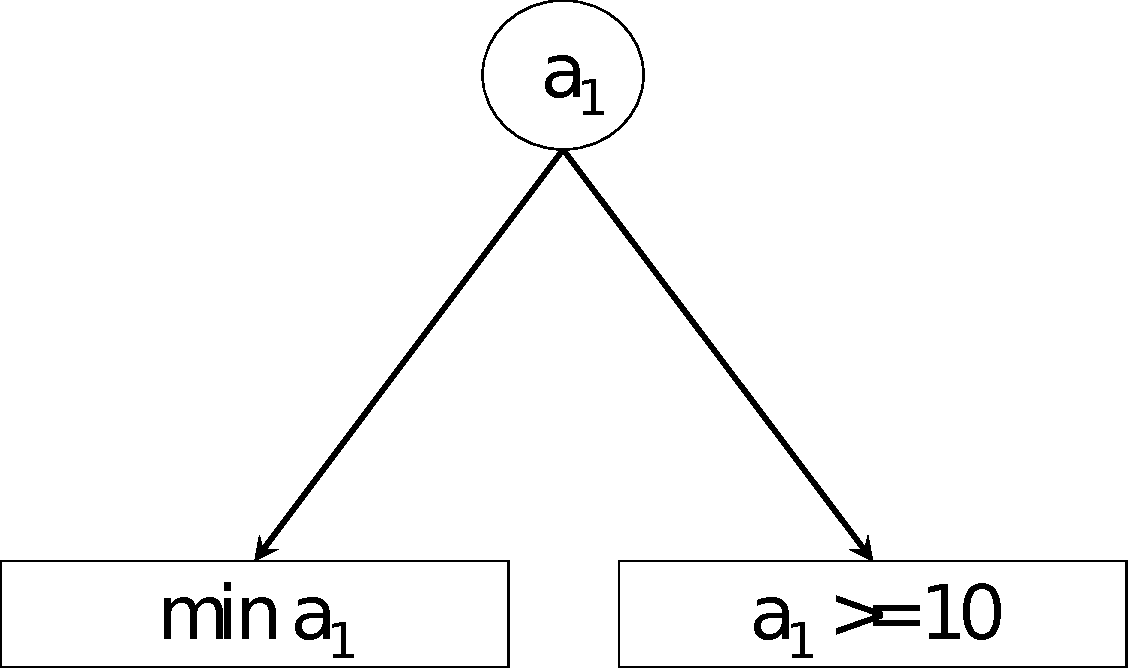
\includegraphics[width=0.4\textwidth]{NCS_conflicting_requests}
\caption{Conflicting trajectories example.}\label{NCS_conflicting_requests}
\end{figure}

When such an agent receives contradictory requests, it needs a way to select which request to apply and which request to reject. We can intuitively see how this decision should be based on the current state of the requesting agents. For example, when receiving requests both a satisfied and a non-satisfied constraint, a variable agent should favor the non-satisfied one. In order for the agents to be able to make this decision, we need to provide them a way to compare the states of different agents.

\paragraph*{Solving Conflicting Requests using Criticality}
To this end, we introduce a new mechanism based on a specific measure called \emph{criticality}. This measure represents the state of dissatisfaction of the agent regarding its local goal. Each agent is in charge of estimating its own criticality and providing it to the other agents\footnote{We do not concern ourselves with the problematic of trust here, each agent is assumed to provide the most trustful and accurate information without cheating or lying. The use of measures such as criticality in open and untrusted environments is in itself an interesting question to say the least.}. The role of this measure is to aggregate into a single comparable value all the relevant indicators regarding the state of the agent. Having a single indicator of the state of the agent is interesting as it simplifies the reasoning of the agents. In addition, this mechanism has the interesting property of limiting the informations transmitted to the others agents, which can be of interest in case of a distributed optimization where data privacy is an issue.
However the system designer has the difficult task to provide the agents which adequate means to calculate their criticality. Also, in specific cases, this information on the state of the agents is not sufficient to take the correct decision, as we will see in the following sections.

In the proposed system, criticality is initially provided by constraint and objective agents and is propagated in the system through their requests.
Let us illustrate this with a constraint of the type \(g(X) \leq t\), with \emph{X} input of the constraint, \emph{g(X)} the constraint equation and \emph{t} the threshold under which the constraint is satisfied. The basic requirements regarding the criticality of this agent is to be low when the constraint is satisfied and high when the constraint is violated. Thus, the criticality of this agent is function of its current value and of the threshold.

\begin{figure}
	\centering
	\begin{subfigure}[b]{\textwidth}
	\centering
	\scriptsize
	
		\[criticality_{t,\eta,\epsilon}(x)=
			\begin{cases}
				0		&\text{if \( x < \; t - \epsilon \) },\\
				-\gamma ( t - x - \eta ) ^ 2 / ( 2 ( \epsilon - \eta)) + \gamma ( t - x - \eta ) + \delta &\text{if \(t - \epsilon \leq \;x \leq \;t - \eta \)},\\
				\gamma (-t-x-\eta)^2/(2 \eta)+\gamma (-t-x-\eta) + \delta &\text{if \(t - \eta \leq \;x \leq \;t\)},\\
				1	&\text{if \( x > \; t \)}
			\end{cases}\]

		where\\
		$\gamma = -2/ \epsilon,$\\
		$\delta = -\gamma (\epsilon - \eta )/2,$\\
		$\text{and } 0 < \eta < \epsilon.$
	\caption{Analytical formulation.}\label{crit_func}
	\end{subfigure}
	
	\begin{subfigure}[b]{\textwidth}
		\centering
		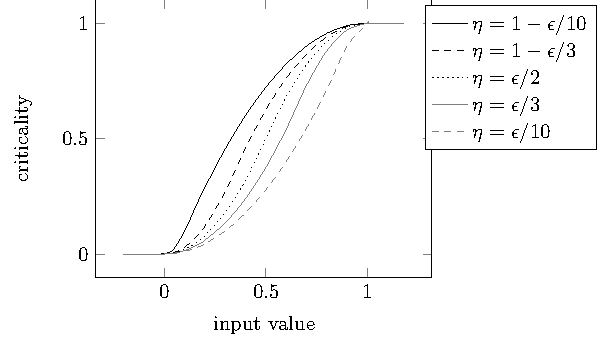
\includegraphics[]{./latex_figs/barrer-fig}
		\caption{Shapes of criticality function of threshold t = 1 for \(\epsilon=1\) and different \(\eta\).}\label{crit_shapes}
	\end{subfigure}
	
\caption{Criticality function of a constraint agent.}
\end{figure}

To compute it, we use the barrier function defined on \figurename{} \ref{crit_func}. It takes as input \(x\), the current value of the constraint. It is parameterized by \(t\), the threshold, and by \(\eta\) and \(\epsilon\) that both regulate the shape of the function as seen on \figurename{} \ref{crit_shapes}. Its value always varies between \(0\) and \(1\).
The \(\epsilon\) can be adjusted by a domain expert if needed: the higher it is, the faster the constraint increases in criticality.
In our experiments, we used $\epsilon = 0.1$ and $\eta$ was set to roughly a third of $\epsilon$, \textit{i.e.} 0.03.
This function allows a smooth transition between two states and provides several interesting properties: it is continuous, differentiable, requires few parameters, is computed quickly and is relatively easy to grasp.

\noindent The criticality of the other agents is determined as follow:

\begin{compactitem}
\item For objective agents: the criticality is set to an arbitrary constant value which must be lower than \(1\). In our experiments we settled for a value of \(0.5\). This translates the fact that, in the general case, an objective could theoretically always be improved, but is less important to satisfy than a constraint.
\item For variable, output and model agents: the criticality is set to the highest criticality among the received requests.
\end{compactitem}

When the system converges to a solution, it stabilizes at a point where the maximum of the criticalities of the agents is minimized.
%%

An illustration on this mechanism can be seen on \figurename{} \ref{NCS_1_conflicting_requests}. In this example, a variable agent (with a current value of 3) receives contradictories requests from an objective (decrease) and a constraint (increase). As the constraint is not satisfied, the criticality associated to its request (0.85) is higher than the one of the objective (0.5). As a consequence the variable agent selects the request of the constraint agent and increases its value.

\begin{figure}
	\centering
	\begin{subfigure}[b]{0.45\textwidth}
		\centering
		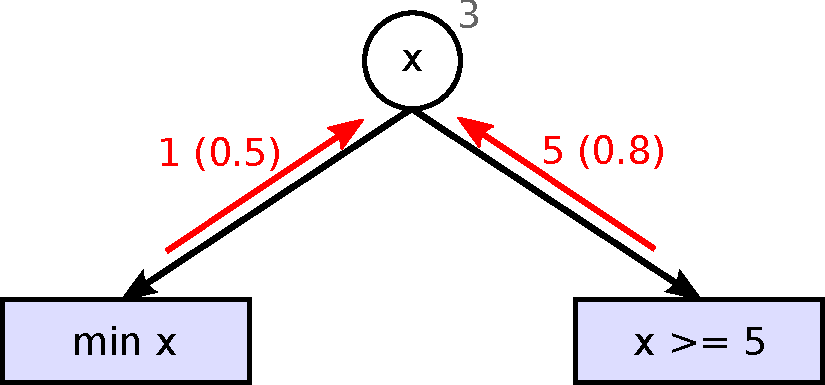
\includegraphics[width=\textwidth]{NCS_1_conflicting_requests_a}
		\caption{The criterions send their requests and current criticalities (in parenthesis).}\label{NCS_1_conflicting_requests_a}
	\end{subfigure}
	\hfill
	\begin{subfigure}[b]{0.45\textwidth}
		\centering
		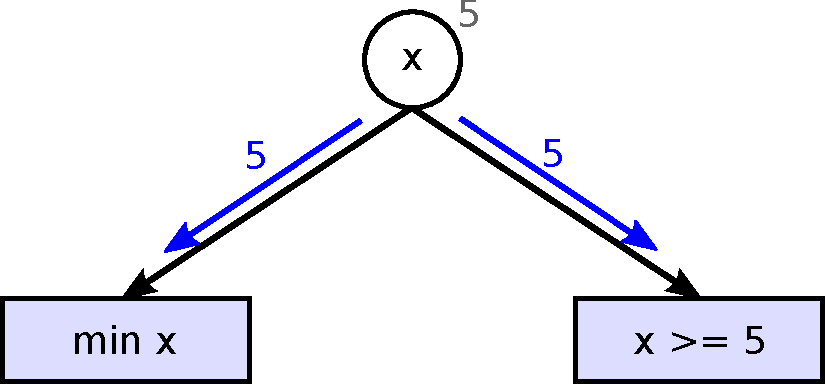
\includegraphics[width=\textwidth]{NCS_1_conflicting_requests_b}
		\caption{The variable agent selects the most critical request and responds accordingly.}\label{NCS_1_conflicting_requests_b}
	\end{subfigure}
	
\caption{Criticality mechanism (the criticality of the requests is indicated in parenthesis).}\label{NCS_1_conflicting_requests}
\end{figure}

\paragraph*{Maintaining a Correct Trajectory with Successive Contradictory Requests}

Another aspect of the handling of contradictory requests concerns the possibility for the agent to receive successively contradictory requests, possibly from the same origin. This situation can arise from the fact that some problem topologies requires the agents to move in a coordinated way across the search space. This difficulty is illustrated on \figurename{} \ref{basin_fun_illustration}. On this figure is presented a 2-inputs functions we want to minimize (top-right corner), and 3 different trajectories. For each of these trajectories, the two inputs vary in the same direction, but with different strengths.\\
We can see that, for the two dashed trajectories, the objective-function increases as the variation of one of the input is much greater than the variation of the other. Only on the non-dashed trajectory the objective is actually improved. The implication is that, even if all the inputs vary in the correct direction, they can cause a degradation of the objective if they do not coordinate the strengths of their variations.

\begin{figure}
\centering
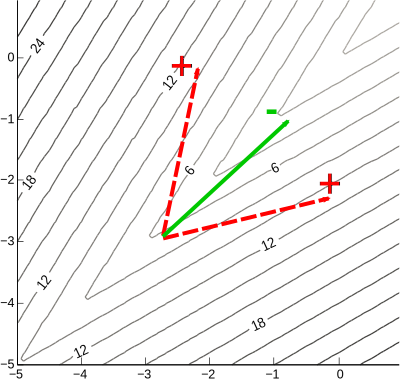
\includegraphics[width=0.4\textwidth]{basin_function_with_trajs}
\caption{Illustration of coordination requirements on a basin function with 3 different trajectories.}\label{basin_fun_illustration}
\end{figure}

With the nominal behavior, the agents would iterate and notice their mistake, compensating by changing direction. However this behavior would lead to a very inefficient trajectory. Consequently it is much more preferable that the variable agents coordinate their respective movements in order to maintain a good trajectory. However, these variable are not related to each others in any way, and cannot communicate with each others. While we could create additional links to make the variables communicate among themselves, it would violate our locality principle. Instead, we propose a mechanism which base itself on the fact that the agents do not directly know each others, but know that the others agents exist and are cooperative. Consequently, by making careful adjustments and observing the feedback of their environment, the agents can be able to estimate the impact of their variation in regard of the variations of the others variable agents, and correct their movement in consequence.

The basic idea is for the variable agent to create a representation of the trajectory it is following (in the 1-dimension space). It uses a \emph{trending trajectory} measure, noted $tt$, whose value varies between -1 and 1. A positive value for $tt$ means that the variable follow an \emph{increase} trajectory, while a negative value implies a \emph{decrease} trajectory. The higher the value of $|tt|$, the stronger the confidence of the agent into the trajectory.

After the variable agent has selected a request, it updates $tt$ based on the direction requested. If the selected request asks the variable agent to decrease, $tt$ is decreased and \emph{vice versa}. The exact impact of the new request on $tt$ is controlled by a trending coefficient noted $\alpha_{trend}$, to which we attributed a value of 0.9, indicating a strong preference for maintaining a consistent trajectory.\\
After updating $tt$, the agent will do the following:
\begin{compactitem}
\item $tt$ if low ($|tt|< 0.1$) or does not contradict the request (both the request and $tt$ indicate the same direction), the request is applied as is.
\item if $tt$ is high ($|tt|> 0.1$) and contradicts the request (the request and $tt$ indicate opposite directions), the agent does not apply the request, choosing instead to not change its value.
\item in the special case where the request asks the agent not to change value, the agent does so whatever the value of $tt$.
\end{compactitem}
This behavior is described in algorithm \ref{algo_speed_coordination}.

\begin{algorithm}
\caption{Conflicting Requests - Speed Coordination}
\label{algo_speed_coordination}
	$r_s \leftarrow$ selected request\;
	\BlankLine
	\tcp{get sign of variation required by current selected request}
	$\Delta_r \leftarrow value_{current} - value_{r_{s}}$\;
	$\sigma_r \leftarrow \left\{
 									\begin{array}{rcr}
 									-1 & if &\Delta_r < 0 \\
 									0 & if &\Delta_r = 0\\ 
 									1 & if &\Delta_r > 0 \\
								\end{array}
								\right.$\;
	\BlankLine
	\tcp{update trending trajectory}
	$tt \leftarrow$ memorized trending trajectory\;
	$tt \leftarrow tt \times \alpha_{trend}	+ \sigma_r(1 - \alpha_{trend})$\;
	\BlankLine
	\tcp{apply the coordination action (using \tablename{} \ref{coord_act})} 
	coordination\_action($tt$, $\sigma_r$)	\;
\end{algorithm}

\begin{table}[htbp]
\caption{Conflicting Requests - Coordination Actions}\label{coord_act}
\centering
\begin{tabular}{lll}
		\toprule
		$\boldsymbol{tt}$ & $>-0.1$ & $< 0.1$\\
		\midrule
		$\boldsymbol{\sigma_r}$ &&\\
		+ & NOMINAL & WAIT\\
		0 & WAIT & WAIT\\
		- & WAIT & NOMINAL\\
		\bottomrule
\end{tabular}
\end{table}

\paragraph*{Anticipating Criticality Variations of Conflicting Requests}

This simple comparison of the criticalities at a given instant is the main way criticality was used in previous application of the AMAS theory. Since the goal of the agents is to reduce the maximal criticality among their neighbors, selecting the request of the most critical neighbor is a basic heuristic to achieve this end. We provide here an additional refinement by making the agents anticipate the effects of their actions on the criticality of the other agents.\\
The agent will memorize the requests and observe how the criticality of the next requests vary based on its actions. From on this observation, the agent makes an estimation of the impact of its action on the criticality of the senders, using the approximation hypothesis that varying in the same direction will cause the same variation of criticality on the senders. These estimations allow the agent to make a prediction on the future criticalities of the senders in the cases where it increases or decreases.

By taking in account not only the \enquote{spacial} aspect (which neighbor has what criticality) but also on the \enquote{temporal} aspect of its action (what will be the consequence of my action on my neighbors), the agent can make a more adequate decision.

The agent deems two requests $r_{max}$ and $r$, where $crit_{r_{max}} > crit_{r}$, to be equivalent in three cases:
\begin{compactitem}
\item When the difference between their criticalities is lower than a given threshold $t_{crit}$\\$|crit_{r_{max}} - crit_{r}|< t_{crit}$.
\item When the predicted difference between their criticalities is lower than $t_{crit}$\\$|(criticality_{r_{max}} + \Delta_{r_{max}}) - (criticality_{r} + \Delta_r)| < t_{crit}$.
\item When the predicted criticality of the least critical request $r$ is greater than the predicted criticality of the most critical one $r_{max}$\\$criticality_{r_{max}} + \Delta_{r_{max}} < criticality_{r}+ \Delta_r$.
\end{compactitem}
This behavior is presented in algorithm \ref{algo_criticality_anticipation}.

(We chose in our experiments to assign the comparison threshold $t_{crit}$ a somewhat arbitrary value of 2\% of the maximum criticality)

Each of these cases represent a situation where the two conflicting agents are reaching an equilibrium state. In these cases the agent cannot simply discriminate using only the criticality information. We will now see in section \ref{coop_traj_descr} an additional mechanism for such cases.

\begin{algorithm}
\caption{Detecting Equivalent Contradictory Requests using Criticality Anticipation}
\label{algo_criticality_anticipation}
	$R \leftarrow $ received requests\;
	$R_{mem} \leftarrow $ the previous memorized requests\;
	
	$t_{crit} \leftarrow$ criticality comparison threshold\;
	\BlankLine
	\tcp{calculate criticality variations}
	\ForEach{$r \in R$}{
		$\Delta_c^r \leftarrow | criticality_r - criticality_{r_{mem}} |$\;
	}
	\tcp{select most critical request}
	$r_{max} \leftarrow \displaystyle\operatorname*{arg\,max}_{r \in R} criticality_r$\;
	\tcp{find equivalent requests}
	$R_{eq} \leftarrow r \in R-\{r_{max}\}: \begin{cases}
															 			&| criticality_{r_{max}} - criticality_{r} | < t_{crit} \\
															 			\text{or} & | (criticality_{r_{max}} + \Delta_{r_{max}}) - (criticality_{r}+ \Delta_r ) | < t_{crit}\\ 
															 			\text{or} & criticality_{r_{max}} + \Delta_{r_{max}} < criticality_{r}+ \Delta_r \\
																\end{cases}$\;
	\BlankLine
	\tcp{update memory}
	$R_{mem} \leftarrow R$\;
\end{algorithm}

\subsection{Cooperative Trajectories}\label{coop_traj_descr}

\subsubsection{For Variable Agents}

This NCS can be seen as an extension of the previous one (conflicting requests). It occurs when a variable agent receives requests from its outputs which lead to contradictory changes on its inputs (\emph{Conflict} NCS). We presented in the previous section how using \emph{criticality} the agent could discriminate between the requests by choosing to satisfy the most critical. However, in some specific cases, this mechanism is not the most efficient. Let us take a simple example, graphically represented in \figurename{} \ref{NCS_cooperatives_trajectories_models}.

Suppose the following problem:

\begin{align*}
\text{Minimize } &2a_1 + a_2\\
\text{Maximize } &a_1 + 2a_2\\
\end{align*}

The graphical representation of this problem is shown in \figurename{} \ref{NCS_cooperatives_trajectories_variables}.

\begin{figure}
\centering
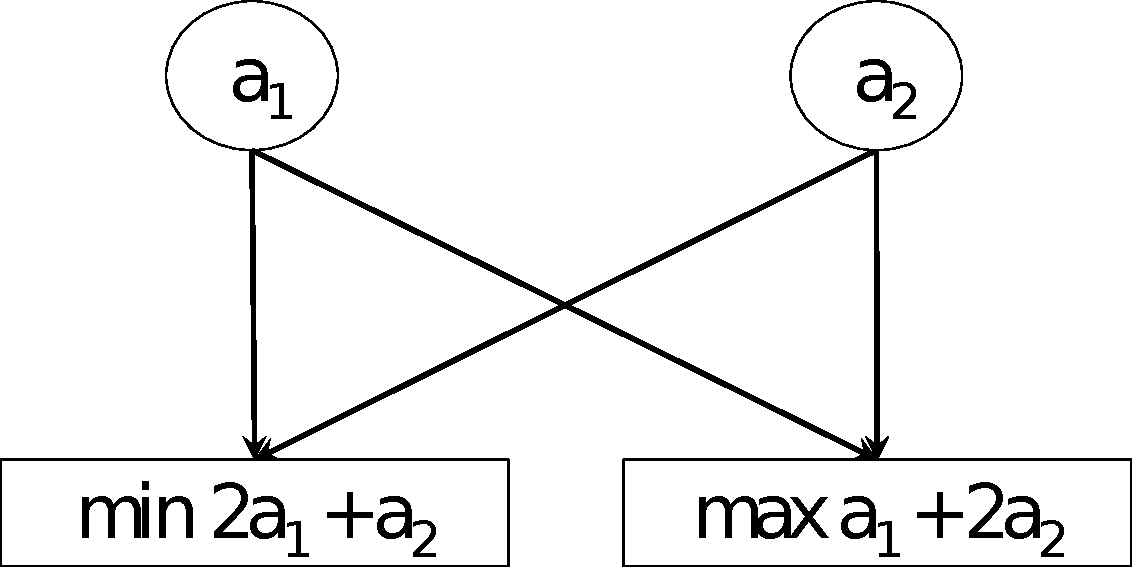
\includegraphics[width=0.4\textwidth]{NCS_cooperatives_trajectories_variables}
\caption{Cooperative trajectories for variable agents example.}\label{NCS_cooperatives_trajectories_variables}
\end{figure}

Using conflicting requests mechanisms, each variable agent would, upon receiving requests coming from the objective and constraint agents, choose to fully satisfy the most critical request, disregarding completely the other. In this example, if the request of $b_1$, the first objective agent, is the most critical, $a_1$ and $a_2$ would both to decrease, they would both to increase if the request of $b_2$, the second objective agent, was the most critical.\\
With this mechanism, the variable agents only have two possibilities: fully satisfy the request of $b_1$, or fully satisfy the request of $b_2$. However we can easily observe how, in this specific problem, the input variables $a_1$ and $a_2$ have different impacts on the two objectives. A variation of 1 for the variable $a_1$ will change the first objective $b_1$ by 2 and the second one $b_2$ by 1, while a variation of 1 for the variable $a_2$ will have the inverse effect.

In such cases, the agents would start by fully helping the most critical to stabilize to a point where the criticalities of both requests are balanced., even if the point is not the most optimal.

\paragraph*{Cooperative Trajectories using Participations}
This observation leads to a third possibility: trying to satisfy both requests at once by satisfying for each variable agent the request on which it has the most \enquote{impact}. Doing so allows a most efficient exploration of the search space by improving several criteria at once. 

This cooperative behavior intervenes only when the variable agent receives multiple contradictory requests with equivalent criticalities (\emph{i.e.}, the agents have reached the point where the criticalities are balanced). In this case, the agent cannot discriminate between the requests using the Conflicting requests cooperative mechanism, as the requests are deemed to be equally important. When the criticalities of the contradictory agents are balanced, the helping agents must now try to improve the situations of both agents \emph{simultaneously}. The goal is to improve the situation of both contradictory agents while keeping the equilibrium.

As the criticalities of the contradictory agents are balanced, the variable agents need an additional information in order to make an adequate action. To do so, we introduce a new measure called \emph{participation}, propagated with the requests exchanged between agent.

The meaning of this measure is the following: when an agent $A$ receives a request from an agent $B$, containing a participation $p$, it means that $B$ estimated the relative impact of $A$ on the request regarding the impact of its others inputs to be $p$ ($p \in [0,1]$).

To estimate the participation, we base ourselves on the correlation estimation mechanism introduced in section \ref{model_agent_solving}. The participation of an agent given by a request is thus calculated as follow:
\begin{compactitem}
\item Constraint/Objective agent: $participation_{i} = \dfrac{| correlation_{i} |}{\displaystyle \sum_{j \in I}{|correlation _{j}|}}$
\item Model agent: $participation_{i,o}\dfrac{| correlation_{i,o} |}{\displaystyle \sum_{j \in I}{|correlation _{j,o}|}} \times participation_{request}$
\item Variable agent: the $participation$ of the received request is propagated as is
\end{compactitem}

When a variable agent receives contradictory requests which are deemed to be of equivalent criticality, it chooses to move in the direction which for which the total participation of the requests is the highest. This behavior is described in algorithm \ref{algo_cooperative_trajectory_variable}.

\begin{algorithm}
\caption{Cooperative Trajectory - Variable Agent}
\label{algo_cooperative_trajectory_variable}
	$R_{equiv} \leftarrow$ selected requests of equivalent criticality\;
	
		$R_- \leftarrow \{r \in R_{equiv} : value_{r} < value_{current}$\}\;
		$R_+ \leftarrow \{r \in R_{equiv} : value_{r} > value_{current}$\}\;
		
		\If{$R_- \neq \emptyset \wedge R_+ \neq \emptyset$}{
			\tcp{select direction with the highest total participation}
			$Part_- = \displaystyle\sum_{r \in R_{-}}{participation_r}$\;
			$Part_+ =\displaystyle\sum_{r \in R_{+}}{participation_r}$\;
	
			\eIf{$|Part_-| > |Part_+|$}
			{
				$R_{selected} \leftarrow R_-$\;
			}
			{
				$R_{selected} \leftarrow R_+$\;
			}
		}
\end{algorithm}

This mechanism allows for several variable agents to make a coordinated action and to improve simultaneously the situation of each requesting agent. Interestingly this coordinated action is made without any explicit communication between the different variable agents, or without these agents even knowing each others existence. The participation measure provides sufficient information to the agent by giving it its relative participation, giving also an implicit information about the relative participation of the \emph{rest of the system}.


\subsubsection{For Model Agents}

We have seen in the previous section how it could be possible in some cases to propose a more efficient exploration of the search space by making variable agents cooperatively adjust their value based on the variation of the different requests they receive. However, if we take the example problem, we can reformulate it as the following equivalent problem:

\begin{figure}
\centering
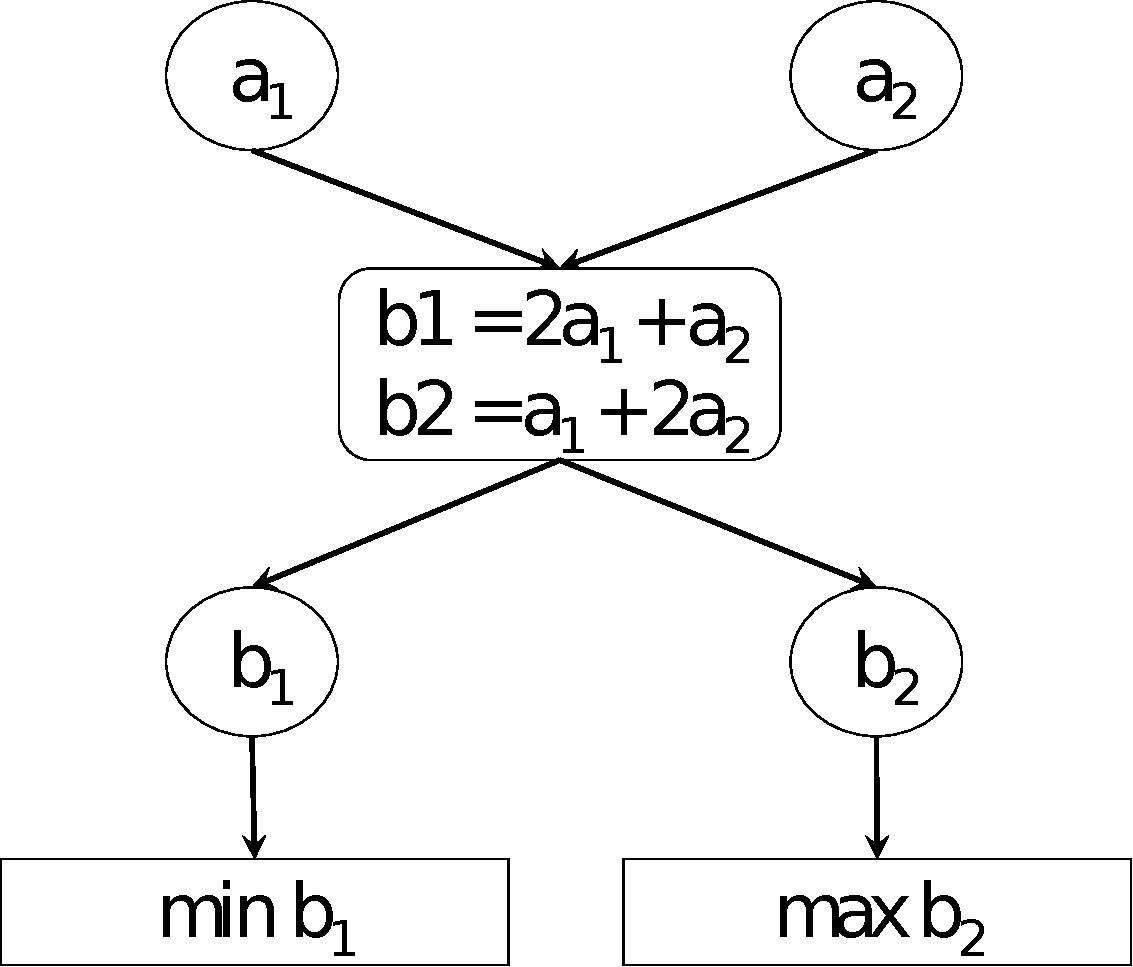
\includegraphics[width=0.4\textwidth]{NCS_cooperatives_trajectories_models}
\caption{Cooperative trajectories for model agent example.}\label{NCS_cooperatives_trajectories_models}
\end{figure}

\begin{align*}
\text{Minimize } &b_1\\
\text{Maximize } &b_2\\
\end{align*}
Where $b_1,b_2$ are outputs of the model $M(a_1,a_2)$ defined as
\begin{align*}
b_1 = &2a_1 + a_2\\
b_2 = &a_1 + 2a_2\\
\end{align*}

Using this new formulation, the model agent will aggregate the requests it receives and only transmit one request to each variable agent. Consequently the variable agents will not be able to perceive the potential cooperative trajectory. In this case, it is the model agent which must detect the possibility of a cooperative trajectory.

To this end, the model agent will use the same mechanisms than the variable agents. First it translates the requests sent by its outputs in requests on its inputs (using the classical propagation mechanisms). Then, for each input, the model agent will take the role of a variable agent and apply the cooperative trajectory mechanism for selecting a request among the requests destined to this input. After a request is selected for each input, the model agent will send the requests to its inputs agents.\\
This behavior is described in algorithm \ref{algo_cooperative_trajectory_model}.

\begin{algorithm}
\caption{Cooperative Trajectory - Model Agent}
\label{algo_cooperative_trajectory_model}
	$I \leftarrow$ the inputs set of the model agent\;
	$R^{out} \leftarrow$ received requests\;
	$O \leftarrow$ associated optimizer\;
	\ForEach{$i \in I$}{
		\tcp{translate received requests into requests on the input}
		$R_i^{in} \leftarrow \{O(r^{out}), \forall r^{out} \in R^{out}\}$\;
		\tcp{apply variable cooperative trajectory on the input}
		\tcp{(as described in algorithm \ref{algo_cooperative_trajectory_model})}
		$r_i^* \leftarrow cooperative\_trajectory(i, R_i^{in})$\;
		\tcp{send the selected request to $i$}
		send($i$, new Request($r_i^*$))\;
	}
\end{algorithm}

\subsection{Cycle Solving}\label{NCS_cycles}

A common difficulty regarding complex optimization problem (and complex systems in general) is the existence of interdependencies (which can be thought as instances of \emph{feedback loops}). For example, for the design of an aircraft, one could try to increase the range of the aircraft by increasing its fuel tank. But doing so, it increases the mass of the aircraft, which in return decreases its range. This complex interdependency between range and mass will appear in the analytical formulation as a cycle in the calculus of the models, \emph{i.e.} to produce its outputs $O_M$, the $Mass$ model will need the outputs $O_R$ calculated by the $Range$ model, taking itself in input the outputs $O_M$ of $Mass$:
\begin{align*}
O_M = &Mass(O_R)\\
O_R = &Range(O_M)
\end{align*}

Such cycles in the problem formulation can pose severe challenge for the optimization process. Once more, we must keep in mind that models must be handled as black boxes; Consequently an analytical solving of the cycle is impossible. Consequently, it is the burden of the agents to detect cycle and take correcting actions of required.

The most basic situation regarding such cycles concerns two directly interdependent models (i.e each one using an output of the other as its input). However, much complex cycles topologies may be encountered. For example, an arbitrary high number of models can be successively chained together in one giant multi-step cycle, or several models can present multiple interdependencies with each other.The solution for which such a cycle is stable (if it exists) is called the \emph{fixed point}.

As the system must work by iterating over these black boxes, the values of the outputs will be iteratively recalculated and propagated between the models involved in the cycle. Depending on the exact structure of the cycle, its effects on the problem solving can be radically different. To illustrate this, let us take the simple following example:
\begin{gather*}
y = a1 \times x \\
x = a2 \times y
\end{gather*}
where \emph{x}, \emph{y} are variables and \emph{a}1, \emph{a2} fixed parameters.
 
The aim is to find coherent values for \emph{x} and \emph{y}. Since models are black boxes, so we cannot directly infer the solution. Depending on the parameters \emph{a1} and \emph{a2} (and excluding the trivial case of \(a1, a2 = 0\)), this structure behaves differently: 
 
\begin{compactitem}
\item \(a1, a2 = 1\): in this case any value for both \emph{x} and \emph{y} satisfies the problem, there is an infinity of fixed points
\item \(a1, a2 < 1\): in this case the system will converge towards the solution. The fixed point is said to be \emph{attractive}
\item \(a1, a2 > 1\): in this case the system will diverge in the opposite direction of the fixed point, which is said to be \emph{repulsive}
\end{compactitem}

The two first cases are benign, and do not impeded the solving process. The third case however will disturb the solving process by moving the state of the system further and further from the stable solution. The task of the agent is then twofold:
\begin{compactenum}
\item detect existing cycles
\item if a cycle is currently diverging, take a correcting action to ensure it converges
\end{compactenum}

An example of diverging cycle is shown in \figurename{} \ref{NCS_cycles_fig}

\begin{figure}
\centering
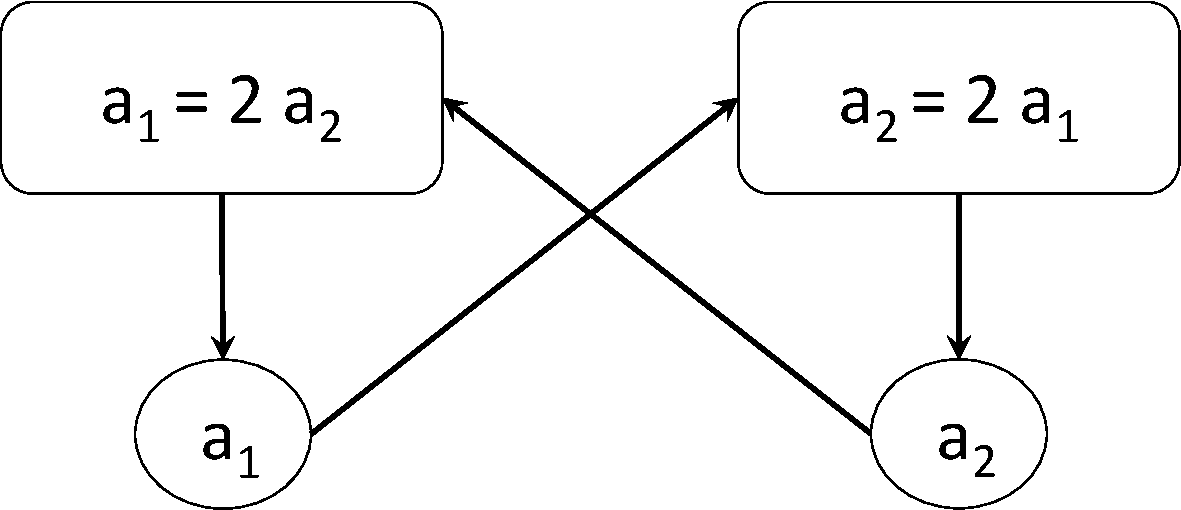
\includegraphics[width=0.4\textwidth]{NCS_cycles}
\caption{Diverging cycle example.}\label{NCS_cycles_fig}
\end{figure}

\paragraph*{Detecting Cycles using Messages Signatures}
To address the detection of cycles, each message is uniquely signed to register its origin. When an agent initiates a message sending by itself (i.e. not as the result of a received message), it \emph{signs} the message with its unique agent \enquote{ID} and an unique message number. The association of these two elements is the \emph{origin signature}.

When an agent sends a message in response to a received message, it adds to the sent message the origin signature of the message causing its action. This way, the signature origin is preserved from message to message and can be used to pinpoint the origin of an activity of the system.

The output agents will be in charge of detecting and handling cycles, as they are in the best position for this. Indeed, being at the junction between criteria and models (or between different models), they are often the ones that can detect cycles the earliest.

To detect a cycle, the output agent creates a correspondence table associating for each origin agent the last signature it received from it. When receiving a message, the agent checks its origin. If the origin agent is not present in the table, the agent adds it. If it is present, it compares the new signature with the one it memorized. If the signatures are different, the agent replaces the old signature with the new one (as the new signature corresponds to a more recent request). If the two signatures match, then there is a cycle.

\paragraph*{Finding Fixed Points}
In case of a cycle, the output agent must now determine if the cycle is converging or diverging towards the fixed point. As in the general case all models are black boxes, the output agent needs to observe the evolution of output values while iterating through the cycle. If the difference between successive values is decreasing, the cycle is converging towards the fixed point, else the cycle is diverging as the variables are going in the \enquote{wrong direction}. To this end, the output agent memorizes the difference between its old and new value, and continues as usual. When receiving the next message from the cycle, it calculates the new difference which enables it to decide if the cycle is converging or not towards the fixed point.

If the cycle is converging, the output agent does not need to do any special action. But in case of a diverging cycle, instead of taking the requested value, the agent emits to its model a request for the opposite direction (\emph{i.e.}, if the value of the output should have increased of \emph{n}, the agent will request a new value corresponding to a decrease of \emph{n}). The request will propagate through the cycle until the fixed point is found.

\subsection{Hidden Dependencies}\label{hidden_deps}

The fact that each agent has only a local and limited view of the problem is a requirement for the system to be able to scale to arbitrary large problems. However this restriction can prove to be problematic when, due to its limited perceptions, an agent makes a wrongful assumption regarding its neighbors. The \emph{hidden dependency} NCS happens when an agent considers that the requests its makes to its input agents are independent while the two agents are in fact dependent. The mistake of the requesting agent comes from the fact that the dependency link between its two input agents is beyond its perception range.

\figurename{} \ref{NCS_hidden_dependencies} is an illustration of a configuration which will lead to a hidden dependency NCS. In this example, the objective agent $\text{min }a_1 + a_2$ will assume that the variable agents $a_1$ and $a_2$ are independent, while the value of $a_2$ is in fact completely dependent from the one of $a_1$ (more precisely $a_2 = -\frac{1}{2} a_1$). In this context, the objective agent will send separate requests to the two variable agents, asking them both to decrease. Since $a_2$ is an output variable, it will transmit the request to its model agent, which will in turn transmit it to $a_1$. And since $a_2$ and $a_1$ are negatively correlated, the transmitted request will ask $a_1$ to increase. Consequently $a_1$ will receive two requests, one (directly from the objective) asking it to decrease, and one (transmitted by $a_2$) asking it to increase.\\
This behavior is described in algorithm \ref{NCS_hidden_dependencies}.


\begin{figure}
\centering
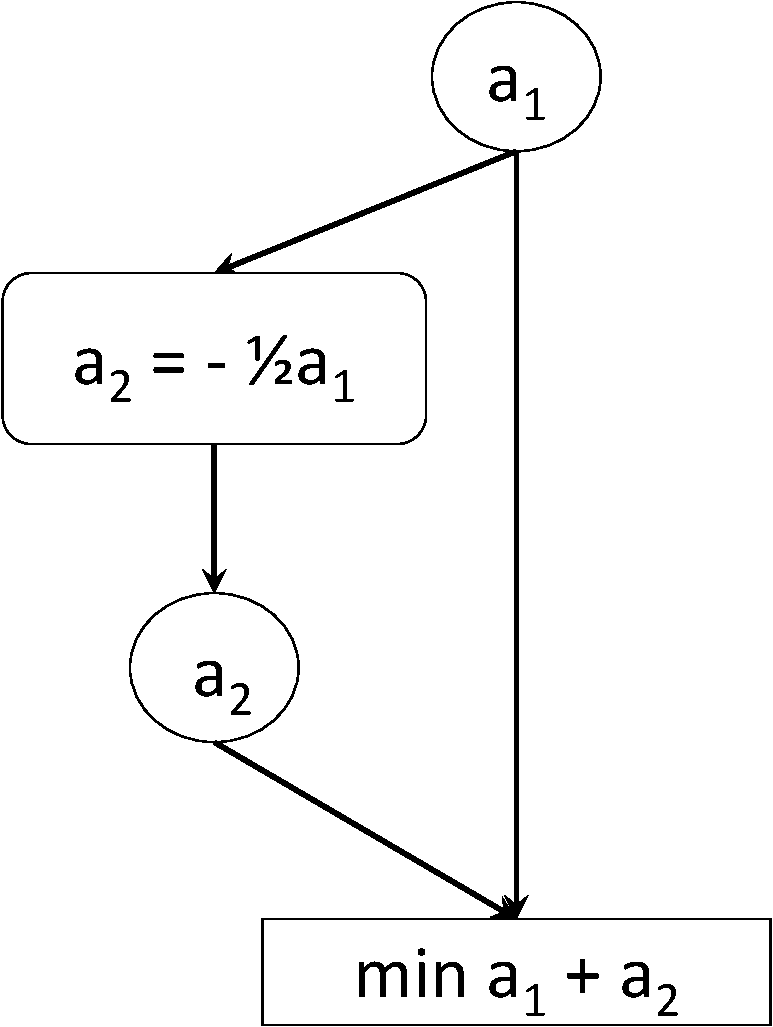
\includegraphics[width=0.3\textwidth]{NCS_hidden_dependencies}
\caption{Hidden dependency example.}\label{NCS_hidden_dependencies}
\end{figure}

This situation is clearly a NCS, as two requests having the same origin should not require an agent to do contradictory actions. We will now propose a mechanism to allow the variable agent $a_1$ to solve the NCS efficiently.

\paragraph*{Detecting Hidden Dependencies with Influences}
First of all the agent must identify the NCS. This part proves to be quite easy using the \emph{origin signature} information we introduced in section \ref{NCS_cycles}. Since every message contains a field recording which agent was at the origin of the request, any agent can know if two requests originate from the same agent by comparing this origin field.\\
In our example, the agent $a_1$ is able to easily detect the NCS, by comparing the two contradictory requests and observing that their origins are the same.

However, our agent still does not know how to solve the NCS as the requests, originating from the same criterion, have identical criticality. To understand what is needed for the agents to be able to solve the problem, let us examine our example again.

In our example, the solution is quite obvious. We want to minimize $a_1 + a_2$, knowing that $a_2 = -\frac{1}{2}a_1$. This problem is then equivalent to minimizing $a_1-\frac{1}{2}a_1$ or, simplified, $\frac{1}{2}a_1$. The correct behavior is thus for $a_1$ to decrease.\\
Let us now change a little this problem, considering instead $a_2$ to be equal to $ -2a_1$. In this case the problem can be rewritten as (after simplifying) minimizing $-a_1$, or maximizing $a_1$. In this case the correct behavior for $a_1$ would be to increase.

It is now obvious that the correct behavior for the agent $a_1$ is extremely dependent on the coefficient of the intermediate model. The same can be said about the coefficients of the objective, and could be said in the general case about any of the intermediate models which could happen to be between the objective and the variable agents. Conceptually, we could say that the variable agent is linked to the objective agent by different \enquote{branches}, with each branch having a specific influence on the objective. In our original example the two \enquote{branches} would have influences of respectively $+1$ and $-\frac{1}{2}$ (and $+1$ and $-2$ in the modified example). That is, the impact of a change of $a_1$ of $\delta_{a_1}$ is of 1 considering the direct branch, and of $-\frac{1}{2}$ considering the branch passing by $a_2$, for a total influence of $\frac{1}{2}$.\\
If we can provide this information to the variable $a_1$, then the agent will be able to solve the NCS by selecting the request coming from the most influent branch(es), ensuring it action will be beneficial for the origin of the requests. We will now see how, by adding a new information with the requests, the agents are able to propagate their local influence to the variable agent, allowing it to solve the NCS.\\
This behavior is described in algorithm \ref{algo_hidden_dependency_influence_propagation}.

\begin{algorithm}
\caption{Influence propagation by internal model agents}
\label{algo_hidden_dependency_influence_propagation}
	\SetKwProg{Bv}{behavior of }{}{}

	\Bv{Objective/Constraint Agent}{
		${c_i} \leftarrow correlations(Inputs, \{output\})$\;
		\tcp{constraint and objective agents have one output only}
		\ForEach{$i \in Inputs$}{
			$influence_{r_i} \leftarrow c_i$\;
		}
	}
	
	\Bv{Model Agent}{
		${c_{i,o}} \leftarrow correlations(Inputs, Outputs)$\;
		\tcp{model agents can have several outputs}
		\ForEach{$r \in$ {selected requests}}{
			\ForEach{$i \in Inputs$}{
				$o \leftarrow sender_r$\;
				$influence_{r_i} \leftarrow influence_r \times c_{i,o}$\;
			}	
		}
	}

\end{algorithm}

\paragraph*{Influence Propagation Mechanism}
Before presenting the exact propagation mechanism, we need to make a quick clarification. In our example, we reasoned on linear models by looking at their coefficients in order to know the different influences. Such reasoning could not be applied to the general black boxes models that the agents use. However, we presented in section \ref{model_agent_solving} a general algorithm which allows the agents to create local linear approximations of any black box models by observing the correlations between the inputs and the outputs of the internal model. Consequently we can assume that each agent with an internal model can always extract the linear factors corresponding to the model, either because they were given to them by the designer, or because they used the aforementioned method to create a local linear approximation (using the observed correlations). During the rest of this section, we will assume that the agents apply the estimation algorithm and use the observed correlations as approximate linear factors of the problem.

To provide the variable agent with the correct influence information, the agents use a simple propagation mechanism. An \emph{influence} field is added to the requests transmitted into the system. The constraint and objective agents which send the original requests fill the influence information with the observed correlation between its output and and the input corresponding to the agent to which the request is sent.\\
An intermediate variable agent will propagate the request without modifying this field, while a model agent will replace it by its old value \emph{multiplied} by the correlation its observed between the output from which it received the request and the input to which the request is sent (this operation is done independently for each input if a request is propagate to several inputs of the model).\\
When a variable agent detect a hidden dependency NCS, it separates the requests coming from the origin in two groups: the requests asking the variable to increase, and the requests asking the variable to decrease. For each group the agent calculates the sum of the influences of each request in the group, then compare the \emph{absolute values} of the total influences. The agent will select the action corresponding to the biggest influence (in absolute value). If the agent is a design variable, it will change accordingly, if it is an output variable it will propagate a request with the same origin and information, but replacing the influence value with the sum of the influences of the winning group.\\
We can say that, in the same way that we \enquote{collapsed} the intermediate models when we wanted to find the solution to our example problem, the intermediate correlations are \enquote{collapsed} into the influence information for the variable agent to be able to solve the NCS.

The detection and solving of a hidden dependency NCS by the variable agents is described in algorithm \ref{algo_hidden_dependency_solving}.

\begin{algorithm}
\caption{Hidden dependency detection and solving by variable agents}
\label{algo_hidden_dependency_solving}

	$R_{received} \leftarrow $ received requests\;
	\tcp{select most critical request}
	$R_{selected} \leftarrow \displaystyle\operatorname*{arg\,max}_{r \in R_{received}} criticality_r$\;

	\If{$|R_{selected}| \geq 2 \wedge \forall( r_1, r_2 \in R_{selected}: origin_{r_1} = origin_{r_2})$}{

		$R_- \leftarrow \{r \in R_{selected} : value_{r} < value_{current}$\}\;
		$R_+ \leftarrow \{r \in R_{selected} : value_{r} > value_{current}$\}\;
		
		\If{$R_- \neq \emptyset \wedge R_+ \neq \emptyset$}{
			\tcp{a conflicting hidden dependency NCS is detected}
			$Inf_- = \displaystyle\sum_{r \in R_{-}}{influence_r}$\;
			$Inf_+ =\displaystyle\sum_{r \in R_{+}}{influence_r}$\;
	
			\eIf{$|Inf_-| > |Inf_+|$}
			{
				$R_{selected} \leftarrow R_-$\;
			}
			{
				$R_{selected} \leftarrow R_+$\;
			}
			handle $R_{selected}$\;
		}
	}

\end{algorithm}

\subsection{Asynchronous Messages}\label{NCS_async}

The last NCS addresses an underlying assumption we have made until now. When we described the behavior of the agents, we supposed each of them always receive the messages in a timely manner, waiting if necessary until all the relevant messages are transmitted before acting. Once again, this hypothetical scenario is made impossible by the need for the agents to maintain a local view. The agents do not know what messages are currently transiting in the system. Their only knowledge concerns the messages they received at the start of their cycle and what messages they previously sent (but not their current status). Consequently, the topology of the agent graph can lead to transmission delays, where messages sent at the same time by the same agent will not necessarily reach their ultimate destination at the same time. For example, let us look back at the hidden dependency example (reproduced on \figurename{} \ref{NCS_hidden_dependencies} for convenience). When we discussed the case of hidden dependencies, we assumed by all the messages sent by the objective agent would reach $a_1$ before the latter would take its decision. However, it is clear that one of the message will take more time to reach $a_1$ than the other, as it must transit by two intermediates. Why would the agent $a_1$ wait for this late message, without even knowing its existence, before acting?

\begin{figure}
\centering
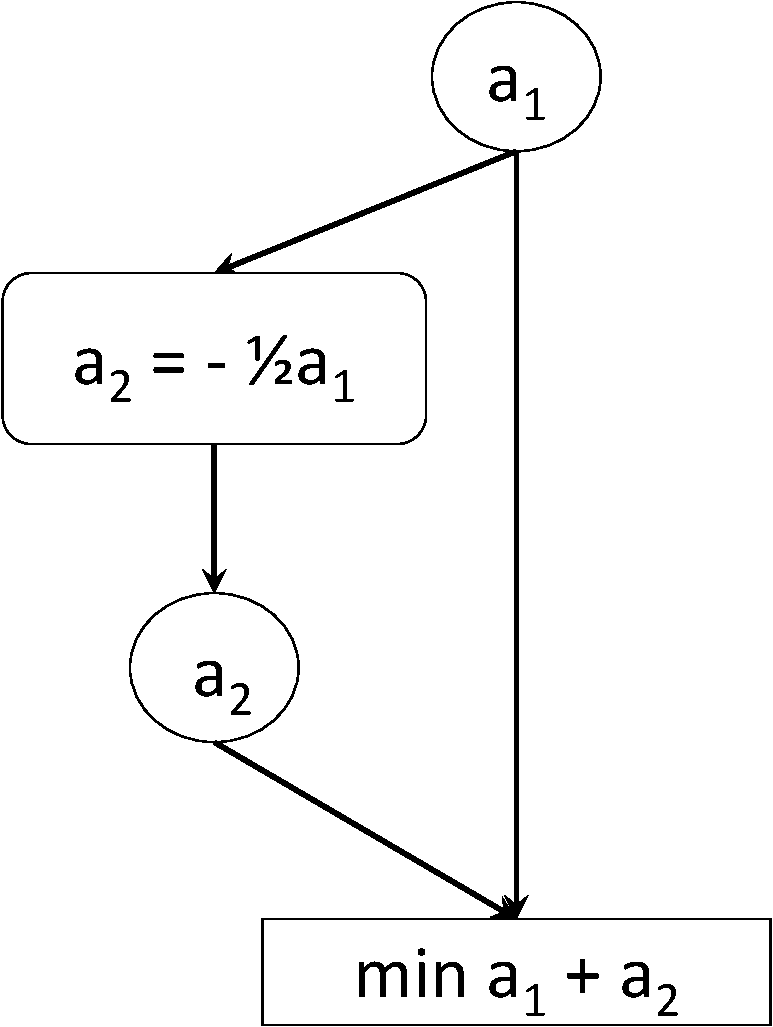
\includegraphics[width=0.3\textwidth]{NCS_hidden_dependencies}
\caption{Hidden dependency example (reproduced).}\label{NCS_async_requests}
\end{figure}

Many of the previous mechanisms we proposed rely on a timely information delivery, for example for the agents to be able to detect some NCS. Based on this, it results that, without an adequate \enquote{synchronization} mechanism, many of them would fail to work correctly. On the other hand, having a fully synchronized system, where all the agents would make lengthy checks to ensure the complete propagation of all messages to all recipients, would be undesirable. Indeed, complex continuous optimization problems create big but loosely connected graphs, for which such full synchronized mechanism would be both costly and inefficient. Moreover, if we take in account the dynamic aspects of the problem (having a designer which can add or remove agent at any moment during solving), obtaining such synchronization guarantee can be nearly impossible.

\paragraph*{Asynchronous Messages with Influences and \emph{allgood} Messages}
We propose a somewhat middle ground mechanism, where the agents try to estimate if they received enough messages to make a correct decision. As some of the information they require is learned during the solving process, an adaptation period will be necessary in order for the agent to behave correctly. During this adaptation period the agents may have a suboptimal behavior where some NCS are not be correctly detected. The iterative nature of the solving process allows these suboptimal decisions to be ultimately corrected by the agents themselves.

The solving mechanism for this algorithm is composed of two parts, regarding how the agents make their estimations for respectively the request messages or the inform messages they expect to receive.
\begin{enumerate}
\item Concerning the requests they expect to receive, the agents base their reasoning on the fact that requests are only sent in answer to previously received inform messages. Consequently they except an answer for the inform messages they previously send. So the agent assume at least one request message by output agent to which it sends an inform message. As the agents are cooperative, each output agent should forward at most one request (the one deemed the most important to handle) back to the agent. Consequently, an agent can expect to receive one and only one request message in response to the informs it send. Once it received a request message from each of its output agents, it can take its decision (either forwarding the most important request to its input(s) or, in the case of a design variable, changing its value and sending new inform messages).\\
The only modification which needs to be done for this mechanism to work concerns (non-criterion) agents which are not linked to any output agents. Previously, when receiving inform messages, these agents would change their value accordingly, but would not send back any message (as they have no request to do). In order for the \enquote{upstream} agents not to be blocked waiting for an answer, an agent that neither has requests to send or informs to forward must answer to its input agent with an \emph{allgood} message, signaling that it has taken into account the inform message and that non other action is pending. An agent receiving such \emph{allgood} message knows that it no longer needs to wait for this output for taking its decision.\\
This behavior is described in algorithm \ref{algo_waiting_requests}.

\item In the same way that an agent waits for requests messages after having sent informs, an agent which has send request messages should wait to receive enough relevant inform messages before taking further steps. In the same way that an agent sending informs expects to receive request messages in return, an agent sending requests expects to receive inform messages in response. A basic solution is thus to apply the same algorithm. In this case however, the agent is not strictly required to wait for all the inform messages to take a relevant decision. We presented in section \ref{model_agent_solving} how the internal model agents can get an indication of the impact of their inputs in regard of their outputs using correlation information. Consequently, such agents can wait until they estimate that they received informs from their inputs corresponding to a total of more than 50\% of the total \enquote{impact} on the value of each output (variables agents, having only one input, always have to wait for this input and this input only, which correspond of 100\% of the total \enquote{impact} on its value).\\
This behavior is described in algorithm \ref{algo_waiting_inform}.
\end{enumerate}

\begin{algorithm}
\caption{Waiting algorithm for request messages}
\label{algo_waiting_requests}

	$O \leftarrow $ \{ outputs \}\;
	$Requests \leftarrow $ \{ received requests \}\;
	$AllGoods \leftarrow $ \{ received allgoods \}\;
	$stillwaiting \leftarrow |Requests| + |AllGoods| \neq |O|$\;

\end{algorithm}

\begin{algorithm}
\caption{Waiting algorithm for inform messages}
\label{algo_waiting_inform}

	$O \leftarrow $ \{ outputs \}\;
	$Informs \leftarrow $ \{ received informs \}\;
	$stillwaiting \leftarrow \forall output \in O, \displaystyle\sum_{info \in Informs}{ influence(input_{info}, output) \leq 50\%}$\;

\end{algorithm}

In our implementation, we did not concern ourself with potential loss of messages, which can happen when the designer intervenes on the system by removing existing agents while messages are transiting. For a \enquote{production-ready} version of the algorithm, such potential losses should be taken into account. Otherwise some agents may hang indefinitely waiting for lost messages. A simple way to remediate to this problem is to add timeouts to the agents. Timeouts are a well-studied problem in computer networks, and adequate algorithms can be proposed based on the works in the existing literature (see \cite{jacobson1988congestion} for example).

\subsection{Summary of Non-Cooperative Situations}

In this section we presented several problematic configurations (NCS) which can arise from the specificities of our modeling of a continuous optimization problem. For each difficulty we presented a basic example of problematic configuration and how this configuration would cause a cooperation failure with the nominal behavior of our agents. The different NCS are summarized in \tablename{} \ref{NCS_summary}

\begin{table}
\caption{Non Cooperative Situations Summary}\label{NCS_summary}
\centering
\begin{tabular}{lp{6.5cm}p{3cm}}
	\toprule
	NCS & Description & Cooperative Mechanisms\\
	\midrule
	Conflicting Requests & An agent receives several incompatible requests & Criticality\\
	Cooperative Trajectories & An agent receives seemingly incompatible requests, which can each be satisfied & Participation\\
	Cycle Solving & Several agents are involved in a diverging cycle & Signature\\
	Hidden Dependencies & An agent sends seemingly independent requests to dependent agents & Signature, Influence\\
	Asynchronous Messages & Agents receive messages in untimely manner & Influence\\
	\bottomrule
\end{tabular}

\end{table}

In each case, we proposed general mechanisms for the agents to be able to detect and correct the NCS in order to maintain a correct and efficient optimization process. In general, we had to provide enough information for the involved agents to detect and correct the NCS. The different mechanisms are summarized in \tablename{} \ref{NCS_mechanisms_summary}

\begin{table}
\caption{Non Cooperative Situations Solving Mechanisms}\label{NCS_mechanisms_summary}
\centering
\begin{tabular}{lp{6cm}p{5.5cm}}
	\toprule
	Mechanism & Description & Properties\\
	\midrule
	Criticality & A aggregated measure to indicate the state of the agent & Comparable between different agents\\
	Signature & A unique signature composed of the unique id of the sender/origin of the message and a (local) timestamp & Comparable, allows a partial ordering of the messages by sender/origin\\
	Influence & An indicator of the impact value of the receiver on the origin & Comparable by origin\\
	 Participation & An indicator of the relative impact of the receiver on the origin relative to the rest of the system & Comparable between different senders\\
	\bottomrule
\end{tabular}
\end{table}

\subsubsection*{Complexity Analysis of Solving Mechanisms}

We now provide a quick complexity analysis of the different solving mechanisms.

\paragraph*{Conflicting Requests}

The main work for solving this NCS consists in finding the request(s) with the highest criticality. This very simple operation can be done by examining each received request in sequence and have a complexity of $\mathcal{O}(n)$ in the number of requests.\\
The solving of this NCS does not require sending additional messages

\paragraph*{Cooperative Trajectories }

When solving this NCS, the agent must group the requests before comparing the total participation of the two groups. The grouping and total participations calculation can be factorized into a single pass algorithm of complexity $\mathcal{O}(n)$ regarding the number of requests.
The agent will not need to send additional messages for solving this NCS.

For models agents, the algorithm will need to be applied on each input, consequently its complexity will be $\mathcal{O}(n \times i)$, $i$ being the number of inputs.

\paragraph*{Cycle Solving}

To detect a cycle, the agent need to compare the signature of each received message with the memorized origin signatures. The complexity of this comparison is $\mathcal{O}(n \times m)$, $n$ being the number of received messages and $m$ being the number of signatures.

\paragraph*{Hidden Dependencies}
When solving this NCS, the agent needs to detect which selected requests come from the same origin, group them, before comparing the total influences of the two groups. The detection, grouping and total influence calculation can all be factorized into a single pass algorithm of complexity $\mathcal{O}(n)$ regarding the number of requests.\\
The agent will not need to send additional messages for solving this NCS.

\paragraph*{Asynchronous Messages}

The algorithm for waiting request is trivial and can be executed in constant time. The algorithm for waiting informs requires a study of every inform for each output, its complexity is thus $\mathcal{O}(n \times o)$, $n$ being the number of informs and $o$ the number of outputs.\\
This mechanism requires the sending of additional messages from (non-criterion) output agents which themselves do not have any output agent. In the best case, there is no such agent, thus no additional message is sent. In the worst case all outputs agent are concerned, and need each to send one additional message (message complexity of $\mathcal{O}(o)$, $o$ being the number of outputs).

\paragraph*{}
It can be seen that, overall, the cooperative mechanisms we proposed to solve the various NCS are quite reasonably efficient in their complexity. This property is important in order for the system to be able to scale to bigger and more complex optimization problem. We managed to keep the complexity of the algorithms low by keeping the reasoning of the agents to a local level, limiting their perceptions to their neighborhood and only very synthetic information about the rest of the system (criticality, origin \emph{etc.}). Moreover, it should be noted that, in many problems, some of the agents will only have a minimal role in the solving, being connected only to one agent in input and one agent in output. For these agents, the complexity of these mechanism will be minimal as they will always receive at most one message. Only in the utmost complex and coupled problems will the majority of the agent be involved in the solving of NCS.

A concern could be raised about the composition of these different mechanisms. Indeed an agent can be involved in several NCS at once. In this case, would not the combination of these mechanisms cause exponential increase of complexity? While this concern could be correct in theory, in practice the different solving mechanisms play the role of successive filters regarding the received messages. Consequently, later mechanisms work on a far lower number of messages than the earlier ones. The typical example is the conflicting requests mechanisms, which will eliminate all the requests which are not deemed critical enough. The others mechanisms will only have to take in account the requests which were conserved by this first filter. More so, it should be noted that, while the different mechanisms have be presented separately, a large part of the processing they do on the messages can be factorized, in order to increase the overall efficiency. While in our implementation we did not do such optimization (in order to keep the mechanisms separated and code easier to work with), such improvements would be of course strongly recommended for a more \enquote{production-ready} implementation of the system.\\
To conclude on this remark, we can safely say that the composition of the different cooperative mechanisms is not of additive complexity, but only bring a marginal increase in the total complexity of the agent behavior.

\chapter{Extending the Multi-Agent System for Uncertainties}\label{mas_uncertainties}

We have seen in section \ref{SOA_uncertainties} how uncertainties can be a major concern in real-life optimization. We have also seen how several types of uncertainties existed and needed to be taken into account. Moreover, complex optimization problems can involve several teams concerned with different disciplines, each of which with its own practices regarding how to manipulate uncertainties, making difficult to study the impact of uncertainties across disciplines.

In this chapter we present a way to alleviate this burden by having the agents automating the uncertainty propagation in the system.

The difficulty is twofold:
\begin{compactitem}
\item \textbf{How do the agents handle uncertainties ?}
How does a model agent calculate the uncertainties on its outputs from the uncertainties of its inputs and its internal model ? How does a constraint agent can handle a probabilistic constraint ?

\item \textbf{How do the agents combine heterogeneous uncertainties modeling ?}
How can a model agent handle inputs with different uncertainties modelings ?
\end{compactitem}

To answer these difficulties we will present a general mechanism inspired by the one we used with external optimizers, which is based on the use of encapsulated external tools to apply the domain-specific expertise.

\section{From Deterministic Optimization to Optimization under Uncertainties}

We previously explained that uncertainties can be present at several levels in the optimization problem. We consider here the two following types of uncertainties:
\begin{compactitem}
\item \textbf{Variable uncertainties}, which are brought by the fact that we cannot perfectly control the value which will be effectively assigned by the design variable.
\item \textbf{Model uncertainties}, which represent the limited precision of the models.
\end{compactitem}

Taking in account these uncertainties leads to a modification of the criteria formulation. Indeed, the constraint $x < 10$ makes sense in the context of deterministic optimization, but not so much when the value of $x$ is uncertain. Is the constraint satisfied when $x$ is an uncertain value, for example represented by an interval ranging from 8 to 12?\\
One can instead propose the following probabilistic constraint $P(x < 10) > 90\%$, which can still be evaluated when manipulating uncertain values. It is possible to propose others criteria formulations manipulating uncertain values, for example one could consider a deterministic constraint concerning the mean of an uncertain variable. Usually, constraints are expressed in a probabilistic form, while objectives use the mean of the variables.

\section{Manipulating Uncertain Values}

Taking in account uncertainties requires modifications at several levels. The most obvious concerns the data structure. On the deterministic version, the data exchanged by the agent were simply real values \footnote{With the obvious limitation of the representation of real numbers on a machine.}. To be able to exchange uncertain values, the agents require a more complex data structure.

As we presented earlier, there are many ways to represent uncertainties, each of them having specific requirements. For example, an interval representation requires two values, the minimum and maximum boundaries, while an uncertainty expressed by a set of measures obtained with Monte Carlos experiments can require the storage of hundreds of thousands points. As we want to maintain the possibility for the designers to choose how they represent uncertainties, we need to provide an abstraction for the agents to be able to consistently handle uncertain values whatever the specific representation.

To this end, we specified the minimum set of operations the agents require. To be able to manipulate an uncertain value, an agent needs to be able to :
\begin{compactitem}
\item obtain the mean of the value (or at least a representative value).
\item obtain the standard deviation of the uncertainty.
\item draw a random value following the law represented by the uncertainty.
\item obtain the cumulative probability of a value (\emph{i.e.} for a given value $t$, what is $P(X < t)$) 
\item obtain the inverse cumulative probability (for a given probability $p$, what is $t$ for which $P(X < t) = p$) associated with the uncertainty).
\end{compactitem}

Any uncertainty representation which can provide these five informations can be used by the system. All the designer needs to do is to provide the module which implements these operations\footnote{The reader familiar the concepts of object-oriented programming and interface implementation will have no difficulty to guess how the process is done in our prototype}.

Let us see how one can provides these information regarding two drastically different modelings: intervals and Monte Carlo experiments.

\paragraph{Intervals Representation}

As the reader knows, an interval representation consist of a lower and upper boundaries. It can be considered as an uniform law, with all the values between the boundaries considered as equally likely. Suppose $l$ and $u$ the boundaries of our uncertainty, we can obtain the required informations using well-known formulas for the uniform law.

\begin{compactitem}
\item the mean can easily be obtained as $\dfrac{u + l}{2}$.
\item the standard deviation is $\sqrt{(u - l)^2 / 12}$.
\item the drawing of a random value consists of drawing a value between $l$ and $u$ using an uniform law, which presents no difficulty.
\item the cumulative probability of $t$ is calculated as $P(X < t) =
			\begin{cases}
				0	&\text{ if t < l}\\
				 \dfrac{t - l }{u - l}	& \text{ if } l < t < u\\
				1	&\text{ if t > u}
			\end{cases}$
\item the inverse cumulative probability of $p$ is obtained as $t = l + p (u - l)$.
\end{compactitem}

As we can see, for a simple representation as intervals the required informations can be obtained very easily.

\paragraph{Monte Carlo Experiments}

The Monte Carlo Experiment is not an uncertainty law \emph{per se} but a series of random drawings to obtain experiment points. If the number of drawings is big enough, then the series can provide an adequate information about the uncertainties governing the variable. Suppose $\{x_n\}$ a series of $n$ drawings over $x$. We suppose the values to be ordered (that is, $x_i < x_j$). 

\begin{compactitem}
\item the mean can be obtained with $\dfrac{1}{n}\displaystyle\sum_n{x_n}$.
\item the standard deviation is obtained by first calculating the variance using the formula $Var(X) = E(X^2) - E(X)^2$ (possible as we can calculate the mean), then taking the square root to obtain the standard deviation.
\item the drawing of a random value consists of drawing a value $i$ between $1$ and $n$ and returning the corresponding point $x_i$
\item the cumulative probability of $t$ is calculated as $P(X < t) = \dfrac{|\{x_i, \forall x_i < t\}|}{|\{x_n\}|}$ (where $|\{x\}|$ is the cardinality of the set $\{x\}$), \emph{i.e.} the number of elements lower than $t$ divided by the total number of elements.
\item the inverse cumulative probability of $p$ is obtained as $ t = x_i$, where $i = p \times  n$.
\end{compactitem}

Even with very specific, non-analytical representation of uncertainties such as datasets from Monte Carlo experiments, we can provide the needed informations without much hassle.

Now that we have defined a common set of operations common to all the uncertainties representations, we can adapt the agents behavior in order to handle them. Such \enquote{uncertainty container} can be associated to variables to represent uncertain values, or to models, indicating uncertainties concerning the underlying model.

For example the designer can estimate that, due to physical limitations, the value of a design variable $x$ cannot be exactly be controlled and will always suffer from an imprecision of +/-0.1 around its assigned value. He can model the uncertainty around the variable with an interval. If he decides to arbitrarily initialize the variable at the value 8, the uncertain value of $x$ will then be [7.9; 8.1].

If the designer observe that the real-world process represented by a specific model tends to produce outputs whose values imprecision can be accurately modeled by a normal distribution, he can associate the normal distribution uncertainty to the model. For example the model $y = 2x$, upon the reception of the information $x = 1$, will produce an uncertain value $y$ with a mean of 2 and a variance corresponding to the associated normal law.

We have now seen how the agents can manipulate uncertainties in isolation. But these mechanisms do not allow the agents to propagate uncertainties in the system. Indeed, if we take our two previous examples, what if the variable $x$ ,associated with an interval uncertainty, is assigned in input of the model $y = 2x$, following a normal distribution? The model has no mechanism to handle uncertainties \emph{received on its inputs}, but these uncertainties must be taken into account as they surely have consequences on the uncertainties of its outputs.\\
The difficulty here is twofold. Not only the model agent must be able to take in account the uncertainties provided by its inputs in addition to its own uncertainty, but it must be able to do so even with uncertainties of different kinds (in our example, interval and normal distribution). We will now present a generic mechanism using \emph{uncertainties propagators} which allows to solve both problems at once.

\section{Uncertainties Propagators}

In the same way we encapsulated expert knowledge on numerical optimization using external optimizers, we propose to encapsulate the knowledge related to the propagation of uncertainties into dedicated modules we call \emph{uncertainties propagators}. While external optimizers are used by the agents to solve local optimization problems, the uncertainties propagators are used by the agents to propagate the uncertainties associated with their inputs and model into uncertainties on their outputs.

The role of an uncertainties propagator is to determine the uncertainties associated with the outputs values of the model based on:
\begin{compactitem}
\item the model itself
\item the uncertainty associated with the model
\item the input values
\item the uncertainties associated with the inputs
\end{compactitem}

As the outputs values cannot be determined by simply evaluating the (deterministic) model, the agent in charge of it will delegate the whole evaluation process to the uncertainties propagator when working with uncertainties. From the agent point of view, an uncertainties propagator is a black box function taking uncertain input values and an uncertain model, and producing uncertain outputs values.

\begin{figure}
\center
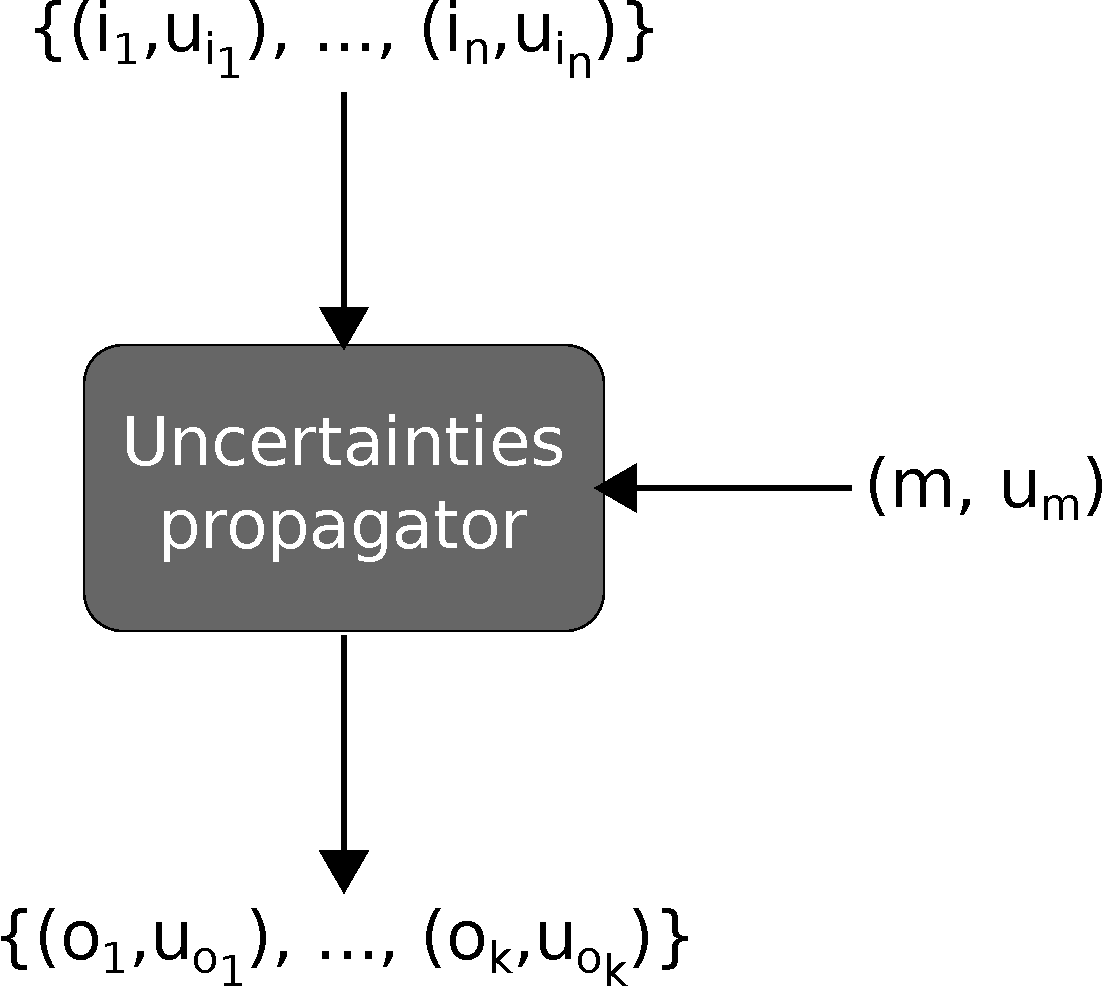
\includegraphics[width=0.4\textwidth]{uncertainties_propagator}
\caption{Uncertainties propagator as a black box function.}\label{uncertainties_propagator}
\end{figure}

\figurename{} \ref{uncertainties_propagator} illustrates the representation of an uncertainties propagator from the point of view of an agent. The uncertainty propagator is a black box. The $(i_j, u_{i_j})$ represent the $n$ uncertain input values of the model (the $i_j$ corresponding to the mean value of the input and $u_{i_j}$ to the associated uncertainty). The model itself $m$ is also provided along with its associated uncertainty $u_m$. Based on the inputs and the model (and their uncertainties), the uncertainty propagator returns the $(o_j, u_{o_j})$ represent the $k$ uncertain output values produced.

This approach shows several advantages. First it allow to keep the functioning of the agents nearly untouched, which in itself is a good sign. Handling uncertain values can be deemed to be an orthogonal concern to the previous ones, and orthogonal concerns should lead to orthogonal changes. Thus this modification of our system to handle uncertainties show that \emph{our modeling is flexible and can be extended easily}.\\
This approach also permit to reduce the work of the designers, which only need to \emph{define the needed propagators once and reuse them} on several problems. This aspect is particularly important as defining a correct way to propagate uncertainties across different disciplines can be an extensive work involving experts from different domains. Providing a way to encapsulate the result of this work in a reusable component leads to a more efficient work process (this concern is especially recognized by software engineers, which created the well-known acronym: DRY - \enquote{Don't Repeat Yourself}).\\
Finally, by strictly encapsulating the required knowledge, we provide a highly modular and adaptable mechanism. \emph{If the needs regarding the modeling of the uncertainties changes, the consequences on the problem are limited solely to the uncertainties representation and/or propagators}. For example, if a designer needs to change the uncertainties associated with a model, he only has to change the uncertainty representation of the model and to use the appropriate propagator (or create it if no adequate propagator already exists).

\section{Conclusion on Uncertainties Handling}

We have seen how the agents can automatically propagate uncertainties in the system, relieving the designers of a part of the burden.\\
This extension to our modeling allow to take in account not only values but uncertain values, that is, values with an associated uncertainty representation. As the exact representation does not concern the agent, these uncertainties are mostly handled as black boxes. In a similar way to how they use optimizers to propagate requests with black box models, internal model agents can use uncertainties propagators to locally propagate uncertainties. In this regard, uncertainties propagators (as well as external optimizers) can be seen as a way to extend the capabilities of the agents provided by the users.

While this mechanism require for the users to provide the uncertainties propagators, it has the advantage that this specific effort has to be done only once, as the resulting propagator can be reusable at will. In this way it can greatly reduce the time different teams need to spend together to overcome the difficulties induced by different working practices. It also open the possibility of propagators libraries, which can be shared and imported as needed.

A note of warning however, the representation of uncertainties is inherently imprecise. In the same way that the modeling of a system contains imprecision, so does the modeling of the uncertainties used to represent this very same imprecision (and so would do the uncertainties used to represent the imprecision on the uncertainties...). Like discussed before, this imprecision is an inherent limitation of the real world. As the uncertainties modeling is in itself factor of uncertainties, it follows that the transformation between two different uncertainties representations will in itself contains some part of imprecision (if only because the passage from one representation to another can lead to information loss, \emph{e.g.} passing from a normal law to an interval modeling).\\
This problematic is not specific to our technique and is indeed present all the same if the uncertainties propagation is done \enquote{manually}. But it is worth reminding, as this complete automation of the propagation could hide it from the mind of the designer.

As a remark we have seen how, by overloading some common mathematical operators, it was possible for the agents to manipulate uncertain values as if they were simple numerical values. Such work could be possibly done with complex numbers, matrix or others, arbitrarily complex, data structures, as long as the corresponding overloaded operators are provided.

\chapter*{Synthesis of the Contribution}

In this part we presented a novel approach for complex continuous optimization using a multi-agent system do distribute the optimization process. We started our work with a new way to model a continuous optimization problem as an agent graph. This modeling allows for an easy and potentially automatic transformation of any problem as a graph, without requiring special knowledge or expertise regarding MAS. Moreover, this transformation does not requires any specific reformulation of the problem, which can keep the natural formulation corresponding to its domain. Because of these properties we named our modeling Natural Domain Modeling for Optimization (NDMO).
\\
To the best of our knowledge, this is the first proposal for providing a common modeling of continuous problems as agents graphs. While we cannot guarantee that is specific modeling will be adopted, it is surely a first step toward opening the field to other contributions. One could wonder if, by dividing the problem into different entities, NDMO would not fall into the same pitfall than MDO methods, applying to the problem a reductionist approach. However, a fundamental distinction is that MDO methods \emph{modify the initial problem in order to reduce its complexity}, while our modeling does not make such modification. On the contrary this modeling fully conserve the interdependencies between the different elements, maintaining an integral and integrative formulation of the problem.

Based on this modeling, we proposed a simple nominal behavior where the agents try to solve individual goals and only has a limited, local perception of their neighbors. These agents can interface with external optimization techniques to solve local optimization problems (or alternatively use some internal optimization mechanisms), and exchange request and inform messages in order to keep a global coherence of the solution. A major distinction with MDO methods is that the global coherence of the problem is not a separate phase but is fully taken in account during the entire process.
\\
While our agents are already able to interface with external optimization methods, some refinements could be proposed. An example could be to, instead of providing each agent with an adequate optimizer, providing all the agents with an optimizer catalog where several optimization methods are presented and characterized. Based on their observation of the manipulated models, the agents could select the optimization method they deem the most appropriate, and even switch between different methods during the solving. Such mechanism would contribute even more to relieving the burden of the designer, but would require to be effective an extensive study of the ontological properties of the field. An other improvement could concerns the internal optimization mechanisms we presented in algorithm \ref{algo_solving_internaloptim}. It could be possible to replace our simple linear approximation estimation by more astute techniques. Such methods could provide more precise estimations to be used by the agents.

This nominal behavior being insufficient to solve some of the issues brought by the specificities of continuous optimization, we use the AMAS theory to identify a set of non cooperative situations, which represent specific patterns of configurations where the nominal behavior of the agents result in a sub-optimal handling of the optimization process. For each of these NCS, we proposed cooperative mechanisms which enrich the nominal behavior of the agent. These additional mechanisms allow to, when necessary, detect and identify the NCS, and to do corrective actions in order to re-establish the correct optimization process.
\\
The AMAS theory has proved to be an effective guide to the conception of our system. By maintaining a local view and concentrating on specific problematic situations, we obtained a behavior which is both scalable and modular. An interesting aspect of this work concerns the different NCS we identified. As our application domain is in itself quite abstracted and general, the NCS we encountered seems themselves to be of a more general nature than in some other works. In chapter \ref{CPSP} we will explore possible uses of this work to other domains than continuous optimization.

We then showed how both our modeling and solving mechanisms are modular enough to be extended in order to handle additional concerns by proposing some modifications which allow to take in account the handling of uncertainties during the optimization process. We detailed the requirements for the agents to be able to handle uncertain values instead of normal numerical values, and we introduced the new concept of uncertainty propagator to provide, using the designers expertise of the uncertainties, an automatic mechanism for propagating heterogeneous uncertainties in the system.
\\
Uncertainties handling is an important concerns in design optimization. As design optimization problems are among the most complex continuous optimization problems, it seemed important to us to provide such functionalities for the system. A quite interesting work would be to propose new ways to extend the system, for example replacing numerical values by vectors, or by extending model agents to manipulate multiple models of different fidelity, experimenting with the possibilities (and the limits) of our proposed modeling.
